\documentclass[12pt]{article}
\usepackage[colorlinks,citecolor=blue,urlcolor=blue]{hyperref}
\usepackage{amsmath}
\usepackage{amsfonts}
\usepackage{amssymb}
\usepackage{graphicx}
\usepackage{enumerate}
\usepackage{natbib}
\usepackage{url} % not crucial - just used below for the URL 
\usepackage{xcolor}
\usepackage{array}
\usepackage{bm}
\usepackage{multirow}
\usepackage{booktabs} 
\usepackage{adjustbox}
\usepackage{caption}
\usepackage{subcaption}
\usepackage{sectsty}
\usepackage{adjustbox}
\usepackage{longtable}
\usepackage[figuresright]{rotating}
\usepackage{multicol}
\usepackage{wrapfig}
\usepackage[plain,noend]{algorithm2e}
\usepackage{bbm}
\usepackage{newtxtext}
\usepackage{amsthm}
\usepackage[subscriptcorrection]{newtxmath}
\usepackage[margin=1in]{geometry}

\newcommand{\blind}{0}
\graphicspath{{./figures/}}

% LaTeX macros

% Last modified: 24/2/2008


%----------------------------------------------
%  A. C. Davison, Institute of Mathematics,
%  EPFL, 1015 Lausanne, Switzerland
%  00 41 21 693 5502
%----------------------------------------------

% mathematical symbols, etc.
\usepackage{environ}
\usepackage{xcolor}

\definecolor{myorange}{HTML}{E24100}
\def\Rev#1{{\textcolor{myorange}{#1}}}
\def\Rem#1{{\iffalse #1 \fi}}
\def\Rep#1#2{{\textcolor{myorange} {#2}}}
\def\r{\color {red}}
\def\rr{\bf\color {red}}
\def\b{\color {blue}}

\NewEnviron{Res}{%
\noindent\textbf{Response: }\textcolor{myorange}{\BODY}
}

\NewEnviron{Comments}{%
\noindent\textsl{\BODY}
}

\newtheorem{lemma}{Lemma}
\newtheorem{theorem}{Theorem}
\newtheorem{proposition}{Proposition}
\newtheorem{corollary}{Corollary}
\newtheorem{definition}{Definition}

\def\dashfill{\cleaders\hbox{-}\hfill}
\def\dashline{\noindent\makebox[\linewidth]{\dashfill}}
\def\r{\color {red}}
\def\rr{\bf\color {red}}
\def\b{\color {blue}}

\def\half{{\textstyle{1\over 2}}}
\def\third{{\textstyle{1\over 3}}}
\def\quarter{{\textstyle{1\over 4}}}
\def\sixth{{\textstyle{1\over 6}}}
\def\frac#1#2{{\textstyle{#1\over#2}}}
\def\Beta{{\rm B}}

\def\argmin{{\rm argmin}}  
\def\diag{{\rm diag}}  
\def\mod{{\rm mod}}  
\def\tr{{\rm tr}}
\def\sign{{\rm sign}}
\def\ow{{\rm otherwise}}  
\def\obs{{\rm obs}}  
\def\endex{{\hfill{\color{red}$\bullet$}\medskip}}
\def\Endex{{\hfill{$\bullet$}\medskip}}
\def\redbf#1{{\color{red}\bf #1}}%
\def\red#1{{\color{red} #1}}%
\def\white#1{{\color{black} #1}}%

\DeclareSymbolFont{AMSb}{U}{msb}{m}{n}
\DeclareMathSymbol{\Natural}{\mathbin}{AMSb}{"4E}
\DeclareMathSymbol{\Integer}{\mathbin}{AMSb}{"5A}
\DeclareMathSymbol{\Real}{\mathbin}{AMSb}{"52}
\DeclareMathSymbol{\Rational}{\mathbin}{AMSb}{"51}
\DeclareMathSymbol{\Imaginary}{\mathbin}{AMSb}{"49}
\DeclareMathSymbol{\Complex}{\mathbin}{AMSb}{"43} 
\DeclareMathSymbol{\Disk}{\mathbin}{AMSb}{"44} 
\def\bi{\begin{itemize}}
\def\ei{\end{itemize}}
\def\bd{\begin{description}}
\def\ed{\end{description}}
\def\ben{\begin{enumerate}}
\def\een{\end{enumerate}}
\def\bv{\begin{verbatim}}
\def\ev{\end{verbatim}}

\def\bth{{$b{\rm th}$ }}
\def\cth{{$c{\rm th}$ }}
\def\dth{{$d{\rm th}$ }}
\def\fth{{$f{\rm th}$ }}
\def\gth{{$g{\rm th}$ }}
\def\hth{{$h{\rm th}$ }}
\def\ith{{$i{\rm th}$ }}
\def\jth{{$j{\rm th}$ }}
\def\kth{{$k{\rm th}$ }}
\def\lth{{$l{\rm th}$ }}
\def\mth{{$m{\rm th}$ }}
\def\nth{{$n{\rm th}$ }}
\def\pth{{$p{\rm th}$ }}
\def\rth{{$r{\rm th}$ }}
\def\sth{{$s{\rm th}$ }}
\def\tth{{$t{\rm th}$ }}
\def\uth{{$u{\rm th}$ }}
\def\vth{{$v{\rm th}$ }}
\def\wth{{$w{\rm th}$ }}

\def\calA{{\mathcal A}}
\def\calB{{\mathcal B}}
\def\calC{{\mathcal C}}
\def\calD{{\mathcal D}}
\def\calE{{\mathcal E}}
\def\F{{\mathcal F}}
\def\G{{\mathcal G}}
\def\H{{\mathcal H}}
\def\calH{{\mathcal H}}
\def\IG{{\mathcal IG}}
\def\cI{{\mathcal I}}
\def\cP{{\mathcal P}}
\def\calJ{{\mathcal J}}
\def\calL{{\mathcal L}}
\def\calK{{\mathcal K}}
\def\calM{{\mathcal M}}
\def\calN{{\mathcal N}}
\def\N{{\calN}}
\def\calP{{\mathcal{P}}}
\def\calQ{{\mathcal{Q}}}
\def\calO{{\mathcal{O}}}
\def\calS{{\mathcal{S}}}
\def\calI{{\mathcal{I}}}
\def\calR{{\mathcal R}}
\def\calT{{\mathcal T}}
\def\calU{{\mathcal U}}
\def\calV{{\mathcal V}}
\def\calW{{\mathcal W}}
\def\calX{{\mathcal X}}
\def\calY{{\mathcal Y}}
\def\calZ{{\mathcal Z}}
\def\W{{\mathcal W}}
\def\U{{\Upsilon}}
\def\f{\frac}
\def\l{{\lambda}}
\def\d{{\delta}}
\def\bX{{\bar X}}
\def\s{{\sigma}}
\def\p{{\partial}}
\def\p{{d}}
\def\v{{\varepsilon}}
\def\dis{{\displaystyle}}
\def\a{{\alpha}}
\def\b{{\beta}}
\def\hash{{\#}}
\def\bar#1{{\overline{#1}}}
\def\hat#1{{\widehat{#1}}}
\def\barY{{\overline{Y}}}
\def\barX{{\overline{X}}}
\def\barZ{{\overline{Z}}}
\def\barx{{\overline{x}}}
\def\bary{{\overline{y}}}
\def\barz{{\overline{z}}}
\def\T{{ \mathrm{\scriptscriptstyle T} }}
\def\mT{{ -\mathrm{\scriptscriptstyle T} }}
\newcommand{\indep}{\perp\!\!\!\perp}
\newcommand{\nindep}{\perp\!\!\!\perp\!\!\!\!\!\!/\;\;}

\newcommand{\med}{{\rm med}}
\newcommand{\card}{{\rm card}}
\newcommand{\bs}{\boldsymbol}
% \newcommand{\do}{{\rm do}}
\newcommand{\Splus}{\textsc{S-Plus}\ }
%\newcommand{\R}{\texttt{R} }

% Bold notation
\def\bR{{\boldsymbol{R}}}
\def\bS{{\boldsymbol{S}}}
\def\bZ{{\boldsymbol{Z}}}
\def\bQ{{\boldsymbol{Q}}}
\def\bN{{\boldsymbol{N}}}
\def\bP{{\boldsymbol{P}}}
\def\bX{{\boldsymbol{X}}}
\def\ba{{\boldsymbol{a}}}
\def\bb{{\boldsymbol{b}}}
\def\bx{{\boldsymbol{x}}}
\def\by{{\boldsymbol{y}}}
\def\bw{{\boldsymbol{w}}}
\def\bs{{\boldsymbol{s}}}
\def\bt{{\boldsymbol{t}}}
\def\bv{{\boldsymbol{v}}}
\def\bu{{\boldsymbol{u}}}
\def\bz{{\boldsymbol{z}}}

\def\real{{\mathbb R}}
%\def\reald{{\mathbb R}^d}

% statistical notation

\def\rmi{{\rm i}}
\def\pr{{\rm Pr}}
\def\Pr{\pr}
\def\E{{\rm E}}
\def\Ev{{\rm Ev}}
\def\var{{\rm var}}
\def\avar{{\rm avar}}
\def\cov{{\rm cov}}  
\def\corr{{\rm corr}}  
\def\Estar{{\rm E^*\thinspace}}
\def\varstar{{\rm var^*\thinspace}}
\def\covstar{{\rm cov^*\thinspace}}  
\def\median{{\rm median}}  
\def\cum{{\rm cum}}
\def\IMSE{{\rm IMSE}}  
\def\AIC{{\rm AIC}}  
\def\BIC{{\rm BIC}}  
\def\NIC{{\rm NIC}}  
\def\AICc{{\rm AIC_c}}  
\def\CV{{\rm CV}}  
\def\GCV{{\rm GCV}}  
\def\IQR{{\rm IQR}}  
\def\MAD{{\rm MAD}}  
\def\Lik{{L}}
\def\logL{{\ell}}
\def\RLik{{RL}}
\def\logLp{{\ell_{\rm p}}}
\def\eqd{{\stackrel{\mathrm{d}}{=}}}
\def\Dto{{\ {\buildrel D\over \longrightarrow}\ }}
\def\dto{{\ {\buildrel d\over \longrightarrow}\ }}
\def\Pto{{\ {\buildrel P\over \longrightarrow}\ }}
\def\rto{{\ {\buildrel r\over \longrightarrow}\ }}
\def\2to{{\ {\buildrel 2\over \longrightarrow}\ }}
\def\Wto{{\ {\buildrel W\over \longrightarrow}\ }}
\def\psto{{\ {\buildrel \rm{p.s.}\over \longrightarrow}\ }}
\def\asto{{\ {\buildrel \rm{a.s.}\over \longrightarrow}\ }}
\def\iid{{\ {\buildrel \rm{iid}\over \sim}\ }}
\def\ind{{\ {\buildrel \rm{ind}\over \sim}\ }}
\def\dotsim{{\ {\buildrel \cdot\over \sim}\ }}
%\def\sim{{\ {\sim}\ }}
%\def\to{{\longrightarrow}}
\def\Deq{{\ {\buildrel D\over =}\ }}
\def\Eoneton{{$E_1,\ldots,E_n$}}
%\def\T1ton{{$T_1,\ldots,T_n$}}
\def\I1ton{{$I_1,\ldots,I_n$}}
%\def\U1ton{{$U_1,\ldots,U_n$}}
\def\X1ton{{$X_1,\ldots,X_n$}}
\def\Y1ton{{$Y_1,\ldots,Y_n$}}
\def\Z1ton{{$Z_1,\ldots,Z_n$}}
\def\R1ton{{$R_1,\ldots,R_n$}}
\def\e1ton{{$e_1,\ldots,e_n$}}
\def\t1ton{{$t_1,\ldots,t_n$}}
\def\x1ton{{$x_1,\ldots,x_n$}}
\def\y1ton{{$y_1,\ldots,y_n$}}
\def\z1ton{{$z_1,\ldots,z_n$}}
%\def\r1ton{{$r_1,\ldots,r_n$}}

% Journal abbreviations

\def\AAP{\emph{Advances in Applied Probability}}
\def\AnnProbab{\emph{Annals of Probability}}
\def\AISM{\emph{Annals of the Institute of Statistical Mathematics}}
\def\AMS{\emph{Annals of Mathematical Statistics}}
\def\ApplStatist{\emph{Applied Statistics}}
\def\AS{\emph{Annals of Statistics}}
\def\B{\emph{Bernoulli}}
\def\Bka{\emph{Biometrika}}
\def\CJS{\emph{Canadian Journal of Statistics}}
\def\CSDA{\emph{Computational Statistics \& Data Analysis}}
\def\Eca{\emph{Econometrica}}
\def\ISI{\emph{International Statistical Review}}
\def\ISR{\emph{International Statistical Review}}
\def\JAMA{\emph{Journal of the American Medical Association}}
\def\JAP{\emph{Journal of Applied Probability}}
\def\JASA{\emph{Journal of the American Statistical Association}}
\def\JBES{\emph{Journal of Business \& Economic Statistics}}
\def\JCGS{\emph{Journal of Computational and Graphical Statistics}}
\def\JSCS{\emph{Journal of Statistical Computation and Simulation}}
\def\JRSSA{\emph{Journal of the Royal Statistical Society series A}}
\def\JRSSB{\emph{Journal of the Royal Statistical Society series B}}
\def\JRSSD{\emph{The Statistician}}
\def\SJS{\emph{Scandinavian Journal of Statistics}}
\def\SPA{\emph{Stochastic Processes and their Applications}}
\def\SM{\emph{Survey Methodology}}
\def\SS{\emph{Statistical Science}}
\def\TAS{\emph{The American Statistician}}
\def\Tech{\emph{Technometrics}}
\def\ZW{\emph{Z. Wahrsch. v. geb.}}
\def\JC{\emph{Journal of Classification}}
\def\PNAS{\emph{Proceedings of the National Academy of Science}}

% utility macros

\def\np{{\newpage}}
\def\gap{{\vskip 0.3in}}
\def\etal{{\sl et al.}} 
\def\pound{{\it \$}}
\def\apriori{{\sl a priori }}
\def\examfoot{{\vfill\hfill{\bf Turn over}\eject}}
\def\newtransparency{{\newpage}}
\def\Section{{Section~}}
\def\Sections{{Sections~}}
\def\Pvalue{{P-value}}
\def\Pvalues{{P-values}}

\def\report#1{{\newpage\centerline{\bf #1}\smallskip}}

% odds and ends

\def\redbf#1{{\color{red}\bf #1}}%
\def\Defn{\redbf{Definition:\ }}%
\def\Thm#1{\redbf{Theorem #1:\ }}%
\def\Ex#1{\redbf{Example #1:\ }}%
\def\Note{\redbf{Note:\ }}%
\def\Exercise#1{\redbf{Exercise #1:\ }}%
\def\Ill{\redbf{Illustration:\ }}%
\def\endex{{\hfill\redbf{$\bullet$}\smallskip}}
\def\calP{{\mathcal{P}}}
\def\calS{{\mathcal{S}}}
\def\calI{{\mathcal{I}}}
\def\eme{{\`eme}}
\def\ere{{\`ere}}
%\def\picbox#1#2{{\centerline{\psfig{figure=#1,height=#2pc}}}}%
\def\picbox#1#2#3{{\centerline{\psfig{figure=#1,height=#2pc,angle=#3}}}}%
\def\tt#1{{\texttt{#1}}}
\def\Der#1{\textbf{D#1}}



\begin{document}

%%%%%%%%%%%%%%%%%%%%%%%%%%%%%%%%%%%%%%%%%%%%%%%%%%%%%%%%%%%%%%%%%%%%%%%%%%%%%%
\title{\bf Fast and efficient inference for flexible spatial extremes models}
\if0\blind{
  \author{Peng Zhong, Scott A.~Sisson, and Boris Beranger \\ 
  UNSW Data Science Hub, School of Mathematics and Statistics,\\ University of New South Wales, Sydney 2052, Australia. \\
  \{peng.zhong, scott.sisson, b.beranger\}@unsw.edu.au}
  \maketitle
} \fi

\baselineskip=25pt
\begin{abstract}
    Statistical modelling of spatial extreme events has gained increasing attention over the last few decades with max-stable processes, and more recently $r$-Pareto processes, becoming the reference tools for the statistical analysis of asymptotically dependent data. Although inference for $r$-Pareto processes is easier than for max-stable processes, there remains major hurdles for their application to very high dimensional datasets within a reasonable timeframe. In addition, both approaches have almost exclusively considered the Brown-Resnick model for its Gaussian foundations and the continuity of its exponent measure. In this paper, we derive a class of models for which this continuity property holds and present the \emph{skewed Brown-Resnick} model, an extension of the Brown-Resnick that allows for non-stationarity in the dependence structure, and the \emph{truncated extremal-$t$}, a refinement of the well-known extremal-$t$ model. We use an inference methodology based on the intensity function of the process which is derived from the exponent measure, and demonstrate the statistical and computational efficiency of this approach. Applications to two real-world problems illustrate valuable gains in flexibility from the proposed models as well as appealing computational gains over reference methodologies. 
\end{abstract}

\noindent{\it Keywords:}  spatial extremes, $r$-pareto process, max-stable process, spectral likelihood.
% \vfill

\baselineskip=25pt

%%%%%%%%%%%%%%%%%%%%%%%%%%%%%%%%%%%%%%%
%%%%%%%%%%%%%%%%%%%%%%%%%%%%%%%%%%%%%%%
%%%%%%%%%%%%%%%%%%%%%%%%%%%%%%%%%%%%%%%
\section{Introduction}
%%%%%%%%%%%%%%%%%%%%%%%%%%%%%%%%%%%%%%%
%%%%%%%%%%%%%%%%%%%%%%%%%%%%%%%%%%%%%%%
%%%%%%%%%%%%%%%%%%%%%%%%%%%%%%%%%%%%%%%

Statistical modelling of spatial extremes has major impacts in the management and assessment of risks inherent to spatial processes. While the univariate extremes framework is well established and easily applicable, modelling the dependence structure in spatial extremes is an active field of research where parametric approaches for asymptotic models face major inferential hurdles and are mostly based on the Brown-Resnick model \citep{Brown.Resnick:1977, Kabluchko.etal:2009}, inhibiting realistic applications in high dimension, $D$. For example, environmental processes are often observed over large regions and/or with fine resolution and having $D$ in the order of thousands is not uncommon. In this manuscript, we demonstrate that these inferential issues can be greatly reduced using spectral density, as long as this density is continuous. We establish conditions for this property to hold and leverage it to construct new flexible models. 

When extreme events are defined as the maxima recorded over a long period of time, max-stable processes \citep{deHaan:1984, Schlather:2002} provide a wide class of models for asymptotically dependent data. However, the likelihood of such models is intractable in high dimensions unless low-dimensional approximations are used, such as the composite (pairwise) likelihood \citep{Padoan.etal:2010,Davison.etal:2012} and the Vecchia approximation method \citep{Huser.Zhong:2023}, which are suitable for dimension up to 1000. A relatively recent alternative spatial modelling framework defines extreme events as the realisations of a process for which a risk functional exceeds some high threshold. The corresponding limiting process are called $r$-Pareto processes \citep{Ferreira.deHaan:2014, Dombry.Ribatet:2015, deFondeville.Davison:2018, deFondeville.Davison:2022} and share the same theoretical foundations as max-stable processes. The likelihood for $r$-Pareto processes is more tractable than for max-stable processes but still requires the evaluation of an intractable exponent function as an normalising constant, which can be avoided by using score matching method \citep{deFondeville.Davison:2018,Lederer.Oesting:2023} or choosing $L_1$-norm as the risk functional. The issues with these pre-mentioned inference approaches are that: the methods based on low-dimensional approximations do not provide reasonable estimates for data with complex dependence structures (nonstationarity, anisotropy) due to their loss of higher-order dependence information; the score matching method for $r$-Pareto processes is computationally unstable and might not converge when the dependence is weak. An alternative likelihood-based inference method, called spectral likelihood, use likelihood function of a limiting multivariate Poisson point process of the max-stable processes \citep{Coles.Tawn:1991,Engelke.etal:2015,Wadsworth.Tawn:2014}, and the same likelihood can be also adopted for the corresponding $r$-Pareto processes by choosing $L_1$-norm as the risk functional. The spectral likelihood is computationally efficient and provides consistent estimates for high-dimensional data with complex dependence structures. However, its computational efficiency needs the assumption that the exponent measure is continuous, which is not always the case for existing models. Likelihood-free alternatives using neural networks \citep{Lenzi.etal:2023} and neural Bayes estimators \citep{Sainsbury.Zammit.Huser:2024, Richards.etal:2024} scale well with large $D$, although they involve a computationally heavy training phase, require fine model tuning and do not provide any statistical guarantees. Almost all of the above references focus on the counterpart of the max-stable Brown-Resnick process, which we call Brown-Resnick $r$-Pareto process for simplicity, due to its simple spectral density and its greater flexibility over other models \citep[see, e.g.,][]{deFondeville.Davison:2018, Richards.etal:2024, Hector.Reich:2024}.          


% \citet{Wadsworth.Tawn:2014} proposed a censoring approach that is more robust but computationally demanding (examples with $D=16$ but can reach $D\approx 30$), motivating the scoring rules based approach of \citet{deFondeville.Davison:2018} that is applicable to scenarios where $D$ is a few thousands. Nevertheless, this gradient scoring approach still requires significant computing power ($\approx$1-6 hours using 16 cores for $D=3,600$ spatial locations) and might not converge when the dependence is too weak. 

We note that max-stable and $r$-Pareto processes both exhibit asymptotic dependence, meaning that they have persisting tail dependence which does not vanish as events become more extremes. Although it can argued that many environmental applications display asymptotic independence \citep[e.g.,][]{Bopp.etal:2021, Huser.Wadsworth:2019} or weakening dependence, it is not always clear whether the process is indeed asymptotically independent or the spatial dependence has simply weakened to some low but positive level, justifying the relevance of such models.

The overarching aim of the research presented here is to define a framework for modelling spatial extremes that allows for a broad class of dependence structures as well as fast and efficient inference. The contributions of this manuscript are multi-fold: we (a) establish theoretical conditions for max-stable and $r$-Pareto models to have a continuous exponent measure; (b) derive two new max-stable and $r$-Pareto models which offer greater flexibility in the dependence structures, where composite likelihood and Vecchia likelihood \citet{Huser.Zhong:2023} fail to capture the local anisotropic dependence structure; (c) provide a fast inference methodology using spectral likelihood that relies on continuity of the exponent measure and is applicable to both model-types; (d) improve the efficiency of state-of-the-art simulation algorithms for $r$-Pareto processes.    

The remainder of the manuscript is organised as follows: Section~\ref{sec:modelling} provides some background on how to model the dependence structure between spatial extremes using max-stable and $r$-Pareto processes while Section~\ref{sec:inference} introduces different strategies to fit parametric models. Once these foundations are established, we provide our theoretical contributions in Section~\ref{sec:theory} which includes the construction of the skewed Brown-Resnick and truncated extremal-$t$ models. Experiments are conducted on synthetic data in Section~\ref{sec:sim} to showcase the efficiency of the proposed inference methodology. Finally, two real data analyses involving fitting the max-stable and $r$ -Pareto models are presented in Section~\ref{sec:real} to illustrate the computational superiority of the proposed methodology over state-of-the-art approaches and to highlight the gains in flexibility of the dependence structure from the skewed Brown-Resnick model over the Brown-Resnick model.  

% high dimensional for logistic and nested (Vettori)
% mostly BR
% not definiing existing events, Davison et al 2012 provide some advice, time to move away from max-stable processes

%%%%%%%%%%%%%%%%%%%%%%%%%%%%%%%%%%%%%%%
%%%%%%%%%%%%%%%%%%%%%%%%%%%%%%%%%%%%%%%
%%%%%%%%%%%%%%%%%%%%%%%%%%%%%%%%%%%%%%%
\section{Modelling approaches for spatial extremes}
\label{sec:modelling}
%%%%%%%%%%%%%%%%%%%%%%%%%%%%%%%%%%%%%%%
%%%%%%%%%%%%%%%%%%%%%%%%%%%%%%%%%%%%%%%
%%%%%%%%%%%%%%%%%%%%%%%%%%%%%%%%%%%%%%%

% Let $X_i(\bs), i=1,2,\ldots$, be independent and identically distributed copies of a real-valued stochastic process $\{X(\bs),\bs\in\calS\}$ with continuous sample paths on the space $\calS \subset \real^2$, and for any finite set of spatial locations $\{\bs_1,\dots,\bs_D\}\subseteq\calS$, let $\bX=(X(\bs_1),\dots,X(\bs_D))^\top$ be the corresponding finite-dimensional random vector.
% % , and $\bm X=(X(s_1),\dots,X(s_D))^\top$ be a $D$-dimensional random vector at , with joint distribution $F$. 
% Note that throughout bold fonts are used to represent vectors unless otherwise stated. 

%%%%%%%%%%%%%%%%%%%%%%%%%%%%%%%%%%%%%%%
%%%%%%%%%%%%%%%%%%%%%%%%%%%%%%%%%%%%%%%
% \subsection{Max-stable processes}
%%%%%%%%%%%%%%%%%%%%%%%%%%%%%%%%%%%%%%%
%%%%%%%%%%%%%%%%%%%%%%%%%%%%%%%%%%%%%%%

% If there exist continuous functions $a_n(\bs)>0$ and $b_n(\bs)\in\real$ such that the limiting process
% %
% \begin{align}
% \label{eq:msp}
% Z(\bs) = \lim_{n \rightarrow \infty} \max_{i=1, \ldots, n} \frac{X_i(\bs) - b_n(\bs)}{a_n(\bs)},
% \end{align}
% has non-degenerate marginals, then $Z(\bs)$ is a max-stable process \citep[][Ch.~9]{deHaan.Ferreira:2006}. The finite-dimensional distribution of $Z(\bs)$, denoted by $G$, is max-stable and therefore its marginals follow the generalized extreme value distribution. 
A max-stable process, $Z$,  with unit Fr\'{e}chet margins can be characterized as
\begin{equation}
\label{eq:spectralrepresentation}
	Z(\bs) = \sup_{i=1}^\infty R_iW_i(\bs),\ \bs\in\calS, 
%    \ R_i \sim \text{PPP}(1/r),\ \text{for}\  r > 0,
\end{equation}
%
where $R_1, R_2, \ldots$, are the points of a Poisson Point Process (PPP) on $(0, \infty)$ 
%with mean measure $\upkappa(\cdot)$ 
and $W_1(\bs), W_2(\bs), \ldots$, independent copies of a stochastic processes $W(\bs)$ on $\calS$ with unit mean \citep{deHaan.Ferreira:2006, Schlather:2002}.
%
The exponent measure restricted onto $\mathbb R^D_+$, denoted by $\upkappa$, can be computed as 
%
\begin{equation}
\label{eq:exponentmeasure}
\upkappa \left([\bm 0,\bm x]^c\right)
= \mathbb E\left[\max_{i=1, \ldots, D} \left\{\frac{W(\bs_i)}{x_i}\right\} \right] 
= \int_0^\infty 1 - \Pr(\bm W \in [\bm 0,\bm xr ])\text dr,	
\quad \bx \in \real_+^D.
\end{equation}
%
where $c$ denotes the complement, and $\bm W=(W(\bs_1),\dots,W(\bs_D))^\top$. As such the distribution function $G$ can be expressed as
\begin{equation}
\label{eq:ppp}
G(\bm x) = \exp\left\{-\upkappa([0,\bm x]^c)\right\} = \exp\left\{-V(\bm x)\right\},
\end{equation}
%
where $V(\bm x)$ is a homogeneous function of order $-1$ called the exponent function. The distribution function $G(x)$ can be also viewed as the probability that no Poisson points of PPP($\upkappa \left([\bm 0,\bm x]^c\right)$) are greater than $\bm x$ at locations $\bs_i,i=1,\dots,D$.     

Depending on the choice of $W$ in \eqref{eq:spectralrepresentation}, the exponent measure $\kappa$ can put mass on the boundaries of $\Omega = R^{D}_+ \setminus \{\bm 0\}$, denoted by $\partial\Omega$, as well as on the interior, $\Omega^\circ = \{\bm x\in \Omega: x_i>0,\forall\ i=1,\dots,D\}$. Let $B_D = \left\{ 1, \ldots, D \right\}$ and $B_k = \left\{ b_1, \ldots, b_k\right\} \subset B_D$, where $b_1 < \cdots < b_k$ such that $\bm x_{B_D} \equiv \bm x$ and $\bm x_{B_k} = \left( x_{b_1}, \ldots, x_{b_k}\right)$. Let $\Omega_{B_k} = \left\{ \bm x \in \Omega: x_j=0\ \text{if}\  j \notin B_k \right\}$, be the subspace of $\Omega$ associated with the components indexed by $B_k$ and $\partial\Omega = \left\{ \Omega_{B_k}, \forall B_k \ \text{and}\ k=1, \ldots, D-1 \right\}$ represent the set of all subspaces of $\Omega$ (i.e., $\Omega = \Omega^\circ \cup \partial\Omega$). Then, the intensity function on each subspace $\Omega_{B_k}$ is given by 
\begin{equation}
    \label{eq:angular_density}
        \lim_{x_i\to 0, i\notin B_k} - V_{B_k}(\bm x),
\end{equation}
where $V_{B_k} = \frac{\partial^k V}{\partial x_{b_1}\dots\partial x_{b_k}}$. The intensity function on $\Omega^\circ$ can be expressed as 
$\kappa(\bm x)= - V_{B_D}(\bm x)$,
where the function $\kappa$ is referred to as the intensity function of the max-stable process as the max-stable process are positive almost surely.

%%%%%%%%%%%%%%%%%%%%%%%%%%%%%%%%%%%%%%%
%%%%%%%%%%%%%%%%%%%%%%%%%%%%%%%%%%%%%%%
% \subsection{$r$-Pareto processes}
% \label{ssec:rpp}
%%%%%%%%%%%%%%%%%%%%%%%%%%%%%%%%%%%%%%%
%%%%%%%%%%%%%%%%%%%%%%%%%%%%%%%%%%%%%%%

The theory of $r$-Pareto processes \citep{Dombry.Ribatet:2015, deFondeville.Davison:2022}, focuses on the limit distribution of stochastic processes deemed extreme according to some risk functional $r(\cdot)$.
Assuming the process $X$ with unit Pareto margins, i.e., $\Pr(X(s)>u)=1/u,u>1$, satisfies the regular varying condition \citep[see][]{Dombry.Ribatet:2015}, i.e., $\lim_{u\to\infty}u\Pr(X/u \in B)=\upkappa(B)$ for all measurable sets $B\subset C^+(\calS)$, where $C^+(\calS)$ is the space of non-negative functions on $\calS$, then the limiting process
%
\begin{align}
\label{eq:rpp}    
\tilde{Z}(\bs) = \lim_{u\rightarrow \infty} \frac{X(\bs)}{u}  \vert r\left(\{X(\bs),\bs\in\calS\} \right) >u,
\end{align}
%
defines a simple $r$-Pareto process on $\calA_r = \left\{ f \in C^+(\calS): r(f) > 1\right\}$ with probability measure $\upkappa(\cdot \cap \calA_r)/ \upkappa(\calA_r)$. The finite dimensional density of the simple $r$-Pareto process is therefore given by
%
\begin{align}
\label{eq:rpp_pdf}
\frac{\kappa(\bx)}{\upkappa(\calA_r^D)}, \bx \in \calA_r^D,
\end{align}
%
where $\kappa$ is the intensity function previously defined and $\calA_r^D$ is the set of $\calA_r$ restricted into $D$ dimensions. 

When in the presence of discontinuities in the exponent measure $\upkappa$ (i.e., presence of mass on the boundaries of the set $\calA_r^D$, denoted by $\partial\calA_r^D$), it means $\tilde Z$ can take values on $\partial\Omega \cap \partial\calA_r^D$. Thus, inference for $\tilde Z$ is computationally challenging since it requires the evaluation of the partial derivatives, $-V_{B_k}(x)$. However, the max-stable process $Z$ does not take values on $\partial\Omega$ almost surely since it is defined as pointwise maxima as in \eqref{eq:spectralrepresentation}. If $X$ is in the maximum domain of attraction of $Z$, ${X_i/n,i=1,\dots,n}$ converges to a Poisson process on $\Omega$ as $n\to\infty$ with mean measure $\upkappa$ \citep[Chapter 6]{Resnick:2006}. This allows for modeling the extremes of $X$ via modeling the Poisson points $\{X_i\}$. Therefore, this approach for modeling $Z$ depends on two convergences, the convergences of $X$ to the Poisson point process and the convergences of $X$ to the max-stable process by taking pointwise maxima, and the fact that $\upkappa$ can put mass on $\partial\Omega$ hurdles the convergences of $X$, thus introduces large bias in the estimates. In this manuscript, we provide conditions ensuring the continuity of $\upkappa$ and introduces two new models.

%%%%%%%%%%%%%%%%%%%%%%%%%%%%%%%%%%%%%%%
%%%%%%%%%%%%%%%%%%%%%%%%%%%%%%%%%%%%%%%
\subsection{Parametric models}
\label{ssec:models}
%%%%%%%%%%%%%%%%%%%%%%%%%%%%%%%%%%%%%%%
%%%%%%%%%%%%%%%%%%%%%%%%%%%%%%%%%%%%%%%

Most of the common models for spatial extremes are initially constructed as max-stable processes from the spectral representation \eqref{eq:spectralrepresentation} and the $r$-Pareto equivalent is then derived.

Letting $W(\bs)=\exp \left(Y(\bs) - \sigma^2/2\right)$ in \eqref{eq:spectralrepresentation}, where $Y(\bs)$ is a Gaussian random process with zero mean and variance $\sigma^2>0$, yields the popular Brown-Resnick model \citep{Brown.Resnick:1977, Kabluchko.etal:2009}. The corresponding distribution function $G$ is given in \citet{Huser.Davison:2013a} while \cite{Wadsworth.Tawn:2014} provides a closed form expression for $V_{B_k}$ as
%
$$
V_{B_k}(\bx) = \Phi_{D-k}\left(\log(\bx_{\bar{B}_k}) - \mu(\bx_{B_k});\Gamma \right) \times f(\bx_{B_k}), \quad \bx \in \real_+^D,
$$
%
where $\bar{B}_k = B_D \backslash B_k$, $\mu(\bm x_{B_k})$ is a linear function of $\log(\bm x_{B_k})$, $\Gamma$ is a positive definite matrix, and $f$ is a function of $\bm x_{B_k}$. When $\bm x_{\bar{B}_k}\to \bm 0$, the value of $V_{B_k}$ goes to zero $\forall B_k\neq B_D$, implying the density of the Brown-Resnick model only places mass on $\Omega^\circ$ (see Corollary~\ref{cor:BR} for its analytical expression) and consequently there are no discontinuities in the exponent measure ($\upkappa\left( \partial \calA_r\right)=0$).

Another possibility is to let  $W(\bs)= \tilde{W}(\bs)_+^\nu / a(\bs)$, where $\tilde{W}_+(\bs) = \max(\tilde W(\bs),0)$, $\tilde W(\bs)$ is a skew-normal process, $a(\bs) = \mathbb{E} \left[ \tilde{W}_+(\bs)^\nu \right]$ and $\nu>0$ is the degrees of freedom, yielding the skew extremal-$t$ model \citep{Beranger.etal:2017} and including the extremal-$t$ model \citep{Opitz:2013} as a special case. \citet{Beranger.etal:2017} derives the analytical expression for the distribution function $G$ and demonstrates the presence of mass in $\partial\Omega$ when $D=3$.
\cite{Beranger.etal:2021} provides the general expression for $V_{B_k}$ \citep[see][for results specific to the extremal-$t$]{Thibaud.Opitz:2015}, indicating the presence of mass on all subspaces of the simplex $\Omega$.

%%%%%%%%%%%%%%%%%%%%%%%%%%%%%%%%%%%%%%%
%%%%%%%%%%%%%%%%%%%%%%%%%%%%%%%%%%%%%%%
%%%%%%%%%%%%%%%%%%%%%%%%%%%%%%%%%%%%%%%
\section{Inference}
\label{sec:inference}
%%%%%%%%%%%%%%%%%%%%%%%%%%%%%%%%%%%%%%%
%%%%%%%%%%%%%%%%%%%%%%%%%%%%%%%%%%%%%%%
%%%%%%%%%%%%%%%%%%%%%%%%%%%%%%%%%%%%%%%

%%%%%%%%%%%%%%%%%%%%%%%%%%%%%%%%%%%%%%%
%%%%%%%%%%%%%%%%%%%%%%%%%%%%%%%%%%%%%%%
% \subsection{Inference methods for max-stable processes}\label{ssec:inf_msp}
%%%%%%%%%%%%%%%%%%%%%%%%%%%%%%%%%%%%%%%
%%%%%%%%%%%%%%%%%%%%%%%%%%%%%%%%%%%%%%%

Assuming some parametric model with parameter vector $\bm \theta \in \Theta$, the density of a max-stable model, $g(;\bm \theta)$, is derived by taking the $D$-fold differentiation of the distribution function \eqref{eq:ppp} which results in a combinatorial explosion and intractability of the likelihood. The most popular solution relies on composite likelihoods \citep{Padoan.etal:2010, Sang.Genton:2014}, with $k$-th order log-likelihood function defined as
%
\begin{equation}
\label{eq:composite}
\ell_{C;k}(\bm \theta;\bm x_1,\dots,\bm x_n)
=\sum_{B_k} \zeta_{B_k} \sum_{i=1}^n\log g(\bm x_{i,B_k};\bm \theta), \quad k< D,
\end{equation}
%
where the first summation is over all subsets of $k$ locations indexed by $B_k$, $\bm x_{i,B_k}$ extracts the $B_k$ components of $\bm x_i$, and $\zeta_{B_k} \geq 0$ are some weights which are often set as binary values based on a fixed cut-off distance between sites. 
Feasible attempts have mostly focused on pairs or triples \citep{Padoan.etal:2010, Huser.Davison:2013a} while \citet{Castruccio.etal:2016} considered higher orders up to $k=11$. The above works conclude that the pairwise likelihood (i.e, $k=2$) offers the best compromise between statistical and computational efficiency.
Alternatives include the Stephenson-Tawn likelihood which makes use of the knowledge of occurrence times of maxima 
\citep{Stephenson.Tawn:2005, Wadsworth.Tawn:2014} and that can be combined to the composite likelihood \citep{Beranger.etal:2021}. The methodology of \citet{Wadsworth:2015} reduces the potentially large bias of the resulting estimators, for moderate dimension $D$. Overall, these approaches require additional information, limited to moderately high dimensions and/or exhibit bias.

Inference for max-stable processes can also be performed via the spectral density \eqref{eq:angular_density}. \citet{Coles.Tawn:1991} introduces the spectral likelihood, where the data $\{\bm X_i,i=1,\dots,n\}$ that are in the domain of attraction of $\bm Z$ can be approximately treated as Poisson points in PPP$(\upkappa(\cdot))$. Assuming the approximation valid for $A_{r_0} = \left\{ \bx \in \real^D_+: \| \bx \|_1 > r_0\right\}$, $r_0>0$, the spectral likelihood is given by
%
\begin{equation}
\label{eq:angular_likelihood_1}
L(\bm x_1,\dots,\bm x_{n_{A}}) 
= \exp\left\{-\upkappa_D(A)\right\} \prod_{i=1}^{n_{A}}\kappa(\bm x_i), 
\end{equation}
%
where $n_A$ is the number of points in $A_{r_0}$ and the proportionality is due to $\upkappa(A_{r_0}) = 1/r_0$ \citep[see also][]{Coles.Tawn:1994}. For parametric models with parameter $\bm \theta \in \Theta$, the spectral log-likelihood is therefore
%
\begin{equation}
\label{eq:angular_likelihood_2}
\ell_A(\bm \theta;\bx_1,\dots,\bx_n) = 
\sum_{i \in \{m: \|\bx_m\|_1 > r_0\}} 
\log \kappa\left( \bm x_i;\bm \theta\right). 
\end{equation} 
%
for some high enough threshold $r_0$. This approaches has been applied to several multivariate extreme value models \citep[see, e.g.,][]{Cooley.etal:2010,Engelke.etal:2015, Beranger.Padoan:2015, Sabourin.etal2013} and in the spatial context to the Brown-Resnick model \citep{Engelke.etal:2015}.
%
Unlike composite likelihood estimates which are asymptotically unbiased and normally distributed, the spectral likelihood estimates are biased since the likelihood function is not the likelihood of the max-stable process itself but of a limiting Poisson process. This issue occurs when events with very small components fall into the region $A_{r_0}$, which can be reduced by introducing censoring \citep[see][]{Wadsworth.Tawn:2014, Thibaud.Opitz:2015}, as well as the approximation is poor due to non-zero mass for $\upkappa$ on the boundaries. Simulation experiments for models with continuous $\upkappa$ in Section~\ref{ssec:par_est} indicates that the bias can be controlled to an acceptable level by appropriately selecting a threshold $r_0$, and is balanced out by significant computational gains. Finally, as indicated in \citet{Thibaud.Opitz:2015}, the likelihood \eqref{eq:angular_likelihood_2} requires that the exponent measure places all its mass in the interior of its domain (e.g., the Brown-Resnick but not the skew extremal-$t$), restricting the range of models that can benefit from this inferential method. This manuscript establishes general conditions for ensuring this property holds and constructs two new models. 

%%%%%%%%%%%%%%%%%%%%%%%%%%%%%%%%%%%%%%%
%%%%%%%%%%%%%%%%%%%%%%%%%%%%%%%%%%%%%%%
% \subsection{Inference methods for $r$-Pareto processes}
%%%%%%%%%%%%%%%%%%%%%%%%%%%%%%%%%%%%%%%
%%%%%%%%%%%%%%%%%%%%%%%%%%%%%%%%%%%%%%%

For $r$-Pareto processes with extremeness defined through $r(\bx_i)>u, i=1, \ldots,n$, the log-likelihood is written as
%
$$
\ell_{rP}\left( \bm \theta; \bx_1, \ldots, \bx_n \right) = \sum_{i \in \left\{ m: r(\bx_m) > u \right\}} \log \left( \frac{\upkappa \left(\bz_m; \bm \theta \right)}{\kappa\left( \calA_r; \bm \theta \right)} \right),
$$
%
where we recall that here $\calA_r = \left\{ f \in C_+(\calS): r(f) \geq 1 \right\}$, and $\bz_{m} = \bx_{m}/u$ represent the realizations of the $r$-Pareto process. The normalising constant, $\kappa\left( \calA_r; \bm \theta \right)$, involves the evaluation of integrals in $\real_+^D$, leading to intractability of the likelihood as the dimension $D$ increases. Simplifications occur when $r(\bx) = x(\bs)$ or $r(\bx) = \sum_{j=1}^D x(\bs_j)/D$ since the constant does not depend on the model parameters, or when $r(\bx) = \max(\bx)$ \citep[see][]{deFondeville.Davison:2018, Dombry.etal:2024}. A such, the spectral likelihood \eqref{eq:angular_likelihood_1} introduced above can be seen as a special for a $r$-Pareto with risk function $r(\bx) = \| \bx \|_1$. 
%
To circumvent the difficulties of computing the likelihood of a $r$-Pareto model, \citet{deFondeville.Davison:2018} propose a score matching approach that no longer requires the evaluation of $\kappa(\calA_r;\bm \theta)$. Weight functions are incorporated to allow to down-weight contributions whose risk is close to the threshold value. Although this approach has mainly been applied to the Brown-Resnick model, it can be used for any model given a careful selection of the weights for those with discontinuities in the exponent measure (such as the skew extremal-$t$).

As suggested by \citet[Proposition 2]{Dombry.etal:2024} (see also Theorem~\ref{thm:r_pareto_simulation}), using rejection sampling, one can generate samples of a $r$-Pareto process with risk functional, $r_2$, from samples of a $r$-Pareto process associated with $r_1$ risk functional as long as $r_2$ is upper bounded by $r_1$ with a constant $M>0$. Consequently, the likelihood of the $r$-Pareto process with the $L_1$ norm risk functional can be used to infer about $r$-Pareto processes with any other risk functional by choosing a high threshold $u>M$ in \eqref{eq:angular_likelihood_2}, in particular for the $L_p$ norm, $p\geq 1$ since all $L_p$ norms are bounded by each other in finite dimensions, $\mathbb R^D$. Indeed, thanks to H\"older's inequality for $L_p$ norms, we have $r_0(\cdot)=\|\cdot\|_1 \leq D^{1-1/p}\|\cdot\|_p,\ p>1$ and therefore can choose $u>D^{1-1/p}, p>1$, to infer the $r$-Pareto process with the $L_p$ norm risk functional using \eqref{eq:angular_likelihood_2} and produce unbiased estimators. This approach has the potential to considerably ease up the computational burden since it does not require the computation of the normalising constant and, to our knowledge, not been considered in the literature yet. 

As previously mentioned, in case of model misspecification and the data only falls into the max-domain of attraction of the model, a censored likelihood approach can help mitigate the bias \citep{Wadsworth.Tawn:2014, Huser.etal:2016} but is limited to $D\leq 30$. When the censored likelihood is out of reach and model misspecification is a significant concern, \citet{Huser.etal:2016} suggest that the block maxima approach is preferred since taking block maxima will artificially increase the tail dependence strength between locations and push the data further towards the fitted dependence model. 
% 
As such, the simulation experiments of Section~\ref{sec:sim} will focus on comparing the performance of the composite and the spectral likelihood for max-stable processes, while for $r$-Pareto processes, the performance of the spectral likelihood will be compared against the score matching method.

%%%%%%%%%%%%%%%%%%%%%%%%%%%%%%%%%%%%%%%
%%%%%%%%%%%%%%%%%%%%%%%%%%%%%%%%%%%%%%%
%%%%%%%%%%%%%%%%%%%%%%%%%%%%%%%%%%%%%%%
\section{Theoretical results}
\label{sec:theory}
%%%%%%%%%%%%%%%%%%%%%%%%%%%%%%%%%%%%%%%
%%%%%%%%%%%%%%%%%%%%%%%%%%%%%%%%%%%%%%%
%%%%%%%%%%%%%%%%%%%%%%%%%%%%%%%%%%%%%%%

%%%%%%%%%%%%%%%%%%%%%%%%%%%%%%%%%%%%%%%
%%%%%%%%%%%%%%%%%%%%%%%%%%%%%%%%%%%%%%%
\subsection{Restricting spatial extreme models to $\Omega^\circ$}
%%%%%%%%%%%%%%%%%%%%%%%%%%%%%%%%%%%%%%%
%%%%%%%%%%%%%%%%%%%%%%%%%%%%%%%%%%%%%%%

To capitalise on the computational potential of the spectral likelihood \eqref{eq:angular_likelihood_1}, we establish general conditions for any max-stable and $r$-Pareto model to concentrate their mass on $\Omega^\circ$. As the intricate relationship between max-stable and $r$-Pareto processes was established in Section~\ref{sec:modelling} and $r$-Pareto models are most often derived from their max-stable counterpart, our approach is taken from a max-stable model perspective.

% First, note that \eqref{eq:exponentmeasure} can be re-written as
% \begin{equation}\label{eq:expfunc1}
% %\upkappa \left([\bm 0,\bm x]^c\right) = 
% V(\bm x) = 
% \sum_{j=1}^D \frac{1}{x_j} \mathbb E\left[W(\bs_j)\mathbbm{1}\left\{ \frac{W(\bs_j)}{W(\bs_i)} \geq \frac{x_j}{x_i},i\neq j \right\} \right] = \int_0^\infty 1 - \Pr(\bm W \in [\bm 0,\bm xr ])\text dr,
% \end{equation}
% where the first equality is most often used to derive the formula of the exponent function \citep{Wadsworth.Tawn:2014, Huser.Davison:2013a} since integrating over the density function of $W$ is much easier than integrating over its probability function as given in the second equality.
%
Recall the exponent function in \eqref{eq:exponentmeasure}, the intensity function of the max-stable process can be expressed as 
\begin{equation}\label{eq:intensity}
	\kappa(\bm x) = -V_{B_D}(\bm x) = \int_0^\infty r^D f_{\bm W}(\bm xr)\text dr,
\end{equation} 
where $f_{\bm W}$ is the joint density function of $\bm W$ and, without loss of generality, the partial derivatives of $V(\bm x)$ with respect to the components in $B_k$ can be obtained through
%
\begin{equation}
\label{eq:partialV_1}
 -V_{B_k}(\bm x) = \int_0^\infty \frac{\partial^k}{\partial x_1\partial x_2\dots \partial x_k}\Pr(\bm W \in [\bm 0,\bm xr ])\text dr. 
\end{equation}
%
By decomposing the joint probability function $\Pr(W\in [\bm 0,\bm xr])$ into a conditional and a marginal component, and assuming its partial derivatives do exist, \eqref{eq:partialV_1} can be re-written as
%
\begin{equation}
\label{eq:partialV_2}
 -V_{B_k}(\bm x) = \int_0^\infty r^k f_{\bm W_{B_k}}(r \bm x_{B_k})  \Pr(\bm W_{\bar{B}_k} \in [\bm 0_{D-k},r \bm x_{\bar{B}_k} ]\ |\ \bm W_{B_k} = r \bm x_{B_k} )\text dr,
\end{equation}
%
where $\bm 0_{D-k}$ is the $D-k$ sub-vector of the zero vector $\bm 0$.
From \eqref{eq:partialV_2}, one can notice that if the conditional probability $\Pr(\bm W_{\bar{B}_k} =\bm 0_{D-k}\ |\ W_{B_k} = \bm x_{B_k} )=0$\ for any $k, 1 \leq k \leq D-1$ and any $\bm x_{B_k} > \bm 0_k$, then the spectral density in \eqref{eq:angular_density} has no mass on $\partial\Omega$. The following theorem formalises this condition. 
%
\begin{theorem}
\label{thm:augular_density}
Let a max-stable process $\{Z(\bs), \bs\in \calS\}$ be defined as in \eqref{eq:spectralrepresentation} with a smooth exponent function $V$ at any finite set of $D$ locations such that the partial derivatives of the function $V$ exist. If and only if the conditional probability of $\bm W$ satisfies the following condition, 
%
\begin{equation}
\label{eq:thm_angular_density}
\Pr(\bm W_{\bar{B}_k}=\bm 0_{D-k} \ |\ \bm W_{B_k} = \bm x_{B_k} )=0,\ \forall\ k \in \{1,\ldots,D-1\},\ \bm x_{B_k}>\bm 0_k \ \text{almost everywhere, }
\end{equation}
%
then the spectral density on $\partial\Omega$, as defined in \eqref{eq:angular_density}, is zero almost everywhere.  
\end{theorem}
%	
The proof of the above theorem can be found in Section~A of the Supplemental Material. This result indicates that the behavior of $V_{B_k}$ on $\partial\Omega$ is determined by the behavior of the process $W$ on its lower-end boundary at zero. Section~\ref{ssec:models} states that for the Brown-Resnick model, we have $W=\exp \left(\tilde{W} - \sigma^2/2\right)$ with $\tilde W$ a centered Gaussian random process. The event $\left\{ \bm W_{\bar{B}_k}=\bm 0_{D-k} \ |\ \bm W_{B_k} = \bm x_{B_k} \right\}$ is  equivalent to the event $\left\{ \tilde{\bm W}_{\bar{B}_k} = -\bm\infty_{D-k} | \tilde{\bm W}_{B_k} = \log(\bx_{B_k}) + \sigma^2/2 \right\}$ and since the conditional distribution of $ \tilde{\bm W}_{\bar{B}_k} | \tilde{\bm W}_{B_k}$ is Gaussian, then \eqref{eq:thm_angular_density} holds, Theorem~\ref{thm:augular_density} confirms the claims that the Brown-Resnick model does not put mass on $\partial\Omega$. Section~\ref{ssec:models} also states that for the skewed extremal-$t$ model, we have $W=\max(\tilde W^\nu,0)$ with $\tilde W$ a skew-normal process and $\nu>0$. The event $\{\bm W_{\bar{B}_k} = \bm 0_{D-k} | \bm W_{B_k} = r \bm x_{B_k} \}$ is equivalent to the event $\left\{\tilde{\bm W}_{\bar{B}_k} \leq \bm 0_{D-k} | \tilde{\bm W}_{B_k} = (r \bm x_{B_k})^{1/\nu} \right\}$, which is not a null event and thus the skewed extremal-$t$ model does indeed put mass on $\partial\Omega$.

%%%%%%%%%%%%%%%%%%%%%%%%%%%%%%%%%%%%%%%
%%%%%%%%%%%%%%%%%%%%%%%%%%%%%%%%%%%%%%%
\subsection{Extending current classes of max-stable and $r$-Pareto models}
\label{ssec:new_models}
%%%%%%%%%%%%%%%%%%%%%%%%%%%%%%%%%%%%%%%
%%%%%%%%%%%%%%%%%%%%%%%%%%%%%%%%%%%%%%%

We now take advantage of Theorem~\ref{thm:augular_density} to construct spatial models that only put mass on $\Omega^\circ$, producing tractable likelihoods. 

%%%%%%%%%%%%%%%%%%%%%%%%%%%%%%%%%%%%%%%
%%%%%%%%%%%%%%%%%%%%%%%%%%%%%%%%%%%%%%%
%%%%%%%%%%%%%%%%%%%%%%%%%%%%%%%%%%%%%%%
\subsubsection{The skewed Brown-Resnick process}
%%%%%%%%%%%%%%%%%%%%%%%%%%%%%%%%%%%%%%%
%%%%%%%%%%%%%%%%%%%%%%%%%%%%%%%%%%%%%%%
%%%%%%%%%%%%%%%%%%%%%%%%%%%%%%%%%%%%%%%

Following the Brown-Resnick construction, to develop max-stable processes with no mass on $\partial\Omega$, one can take the exponential marginal transformation of a process with a light marginal tail that places zero mass on the infimum of its marginal marginal space, $\real$ such that the transformed space will have support $[0, \infty]$. The following theorem extends the Brown-Resnick process by considering the extended skew-normal distribution (see Definition~1 in Section~B of the Supplementary Material).

\begin{theorem}
\label{thm:skewBR}
Let $W(\bs) = \exp \left\{ Y(\bs) - a(\bs)\right\}$ where $Y(\bs)$ is a centred skew-normal process with scale matrix $\Sigma$ and slant parameter $\bm \alpha$, and $a(\bs) = \log \mathbb{E} \left[ \exp\left\{ Y(\bs) \right\}\right]$.
The corresponding max-stable process defined via \eqref{eq:spectralrepresentation} is called the skewed Brown-Resnick process and is characterized by the following exponent function:
%
\begin{equation}
\label{eq:V_skBR}
V(\bm x) =\sum_{k=1}^D \frac{1}{x_k} 
\Psi \left(\log \left( \frac{\bm x^{\circ\circ}_{-k}}{x^{\circ\circ}_k} \right) + \frac{\tilde{\bm \omega}_{-k}^2 - \tilde{\omega}_k^2 \bm 1_{D-1}}{2} ; \bm \mu_k, \Sigma_k, \hat{\bm \alpha}_k, \tau_k \right),
\end{equation}
%
where 
$\bm x^{\circ\circ} = \left( x^{\circ\circ}_1, \ldots, x^{\circ\circ}_D\right)$, 
$x^{\circ\circ}_k = 2x_k \Phi\left( \tau_k; 0, 1 \right), k=1, \ldots, D$, 
$\tau_k = \tilde{\omega}_k \delta_k$, $\tilde{\bm \omega} = \left( \tilde{\omega}_1, \ldots, \tilde{ \omega}_D\right) = \omega \bm 1$, $\omega = \sqrt{\diag(\Sigma)}$, 
% $\omega_{[k]}$ is the diagonal element of $\omega$ with index $k$, 
$\bm \delta = \left( 1 + \bm \alpha^\top \bar{\Sigma} \bm \alpha\right)^{-1/2}\bar{\Sigma} \bm \alpha$, 
$\bar{\Sigma} = \omega^{-1} \Sigma \omega$,
$\bm\mu_k = A_k \Sigma_{\cdot k}$, 
$A_k = (\bm e_1, \ldots,\bm e_{k-1}, -\bm 1,\bm e_{k},$ $\ldots,\bm e_{D-1})$, 
$e_k$, $k=1, \ldots, D-1$ are standard basis vectors of dimension $(D-1)$, 
% $a_k = \log(2) + \omega_k^2/2 + \log \Phi(\xi_k;0,1)$, $\bm\xi = \frac{\Sigma\bm\eta}{\sqrt{1+\bm\eta^\top\Sigma\bm\eta}}$, 
$\Sigma_k = A_k \Sigma A_k^\top$, 
$\hat{\bm\alpha}_k = \left(1-\bm\delta^\top \omega A_k^\top\Sigma_k^{-1} A_k \omega\bm\delta \right)^{-1/2} \hat{ \omega}_k\Sigma_k^{-1}A_k \omega\bm\delta$, 
% $\bm \delta = \frac{\bar{\Sigma}\bm\alpha}{\sqrt{1+\bm\alpha^\top\bar{\Sigma}\bm\alpha}}$, 
and $\hat{\bm \omega}_k = \sqrt{\diag(\Sigma_k)}$.
\end{theorem}

\begin{proposition}
\label{prop:AngDesn_skBR}
The skewed Brown-Resnick model defined in Theorem~\ref{thm:skewBR} has zero mass on $\partial\Omega$ and its density on $\Omega^\circ$ is given by
%
\begin{multline}
\label{eq:h_skBR}
\kappa(\bm x) =\frac{2\Phi(\tilde{\tau};0,1)| \Sigma |^{-1/2} \left( \bm 1^\top \bm q\right)^{-1/2}}{\left( 2\pi \right)^{(D-1)/2}\prod_{k=1}^D w_k}\exp \left\{ -\frac{1}{2} \left[ \log \bm x^{\circ\circ\top} \calM \log \bm x^{\circ\circ} + \log \bm x^{\circ\circ\top} \left( \frac{2 \bm q}{\bm 1^\top \bm q} + \calM\tilde{\bm\omega}^2\right) + \right.\right. \\ 
\left.\left. \frac{\bm q^\top\tilde{\bm \omega}^2 - 1}{\bm 1 ^\top \bm q} + \frac{1}{4}\tilde{\bm\omega}^{2,\top}\calM\tilde{\bm\omega}^2 \right]\right\},
\end{multline}%
where $\bm q = \Sigma^{-1} \bm 1$, $\calM = \Sigma^{-1} - \bm q \bm q^\top / \bm 1^\top \bm q$ and  
$$\tilde{\tau}=\left(1 + \frac{\left(\alpha^\top\omega^{-1}\bm 1\right)^2}{\bm 1^\top \bm q} \right)^{-1/2} \bm\alpha^\top\omega^{-1}\left[\left(\mathbb{I} - \frac{\bm 1\bm q^\top}{\bm 1^\top \bm q}\right)\left(\log \bm x^{\circ\circ} + \frac{\tilde{\bm\omega}^2}{2}\right) +  \frac{\bm 1}{\bm 1^\top\bm q}  \right].$$
\end{proposition}

As argued by \citet[][Section~5.2]{Azzalini:2013}, inference involving the extended skew-normal distribution can be improved through the re-parametrisation $\bm \eta = \omega^{-1} \bm \alpha$. As such, we have $\omega \bm \delta = \Sigma \bm \eta \left( 1+\bm \eta^\top \Sigma \bm \eta\right)^{-1/2} \equiv \bm \xi$, and in \eqref{eq:V_skBR} and \eqref{eq:h_skBR} we get $\tau_k = \xi_k$ and $\hat{\bm\alpha}_k = \left(1-\bm\xi^\top A_k^\top\Sigma_k^{-1} A_k \bm\xi \right)^{-1/2} \hat{ \omega}_k\Sigma_k^{-1}A_k \bm\xi$. The proofs of Theorem~\ref{thm:skewBR} and Proposition~\ref{prop:AngDesn_skBR} are relegated to Section~C.1 and C.2 of the Supplementary material where the above re-parametrisation is also introduced to highlight the reduction in computational complexity of evaluating \eqref{eq:V_skBR}. Section~C.3 provides the partial derivatives of the exponent function, required to compute the density of the corresponding $r$-Pareto process. 

\begin{corollary}
\label{cor:BR}
Setting $\bm \alpha = 0$ (or equivalently $\bm \xi=0$), implies $\hat{\bm \alpha}_k = \bm 0$, $\tau_k=0$ and therefore $\bm x^{\circ\circ} = \bm x$, recovering the Brown-Resnick model, where \eqref{eq:V_skBR} and \eqref{eq:h_skBR} reduce to the expressions respectively given in \citet{Huser.Davison:2013a}
% , and from \eqref{eq:h_skBR} the corresponding spectral density on $\Omega^\circ$ is given by
% %
% \begin{multline}
% \label{eq:h_BR}
% h(\bm w) =\frac{| \Sigma |^{-1/2} \left( \bm 1^\top \bm q\right)^{-1/2}}{\left( 2\pi \right)^{(D-1)/2}\prod_{k=1}^D w_k}\exp \left\{ -\frac{1}{2} \left[ \log \bm w^{\top} \mathcal{A} \log \bm w + \log \bm w^{\top} \left( \frac{2 \bm q}{\bm 1^\top \bm q} + \calA\tilde{\bm\omega}^2\right) + \right.\right. \\ \left.\left. \frac{\bm q^\top\tilde{\bm \omega}^2 - 1}{\bm 1 ^\top \bm q} + \frac{1}{4}\tilde{\bm\omega}^{2,\top}\calA\tilde{\bm\omega}^2 \right]\right\},
% \end{multline}%
% %
% which is identical to the result from 
and \citet{Wadsworth.Tawn:2014} without assuming constant variance.
\end{corollary}

Both the matrix $\calM$ and $\mathbb{I} - \frac{\bm 1\bm q^\top}{\bm 1^\top \bm q}$ given in Proposition~\ref{prop:AngDesn_skBR} are singular with a null space $\{c\bm 1:c\in\mathbb R\}$, which makes the model less identifiable for the slant parameter $\bm \alpha$, in particular when using the spectral density. The condition $\bm \eta^\top \bm 1 = \bm \alpha^\top \omega^{-1}  \bm 1 = \bm 0$ is therefore imposed to improve the identifiability of the skewed Brown-Resnick process. Similar conditions were applied by \citet{Padoan:2011} and \citet{Beranger.etal:2019} when considering skewed versions of the H\"{u}sler-Reiss model, the multivariate equivalent of the Brown-Resnick model. 

%%%%%%%%%%%%%%%%%%%%%%%%%%%%%%%%%%%%%%%
%%%%%%%%%%%%%%%%%%%%%%%%%%%%%%%%%%%%%%%
%%%%%%%%%%%%%%%%%%%%%%%%%%%%%%%%%%%%%%%
\subsubsection{The truncated extremal-$t$ process}
%%%%%%%%%%%%%%%%%%%%%%%%%%%%%%%%%%%%%%%
%%%%%%%%%%%%%%%%%%%%%%%%%%%%%%%%%%%%%%%
%%%%%%%%%%%%%%%%%%%%%%%%%%%%%%%%%%%%%%%

This section explores how to remove the density mass on $\partial\Omega$ of the extremal-$t$ process by imposing a truncation on the original process $W(\bs)$. For simplicity we focus on the extremal-$t$ model but similar results can be derived for the skewed extremal-$t$.  

\begin{theorem}
\label{thm:truncated_extremal_t}   
Let $W(\bs) = \tilde{Y}(\bs)^\nu / a(\bs)$, where $\tilde{Y}(\bs) = Y(\bs)|Y(\bs)>0$, $Y(\bs)$ is a centred Gaussian process with unit variances and correlation matrix $\Sigma$, and $a(\bs) = \mathbb{E}\left[ \tilde{Y}(\bs)^\nu\right]$, $\nu>0$.
The corresponding max-stable process defined via \eqref{eq:spectralrepresentation} is called the truncated extremal-$t$ process and is characterized by the following exponent function:
%
\begin{equation}
\label{eq:V_tet}
V(\bx) = \sum_{k=1}^D \frac{T_{\nu+1}^\circ\left( \left(\frac{\bm x_{-k}^\circ}{\bm x_{k}^\circ}\right)^{1/\nu} ;\Sigma_{-k,k},\frac{\mathbb{I}_{D-1}-\Sigma_{-k,k}\Sigma_{k,-k} }{\nu+1}\right)}{\bm x_k T_{\nu+1}^\circ\left(\bm \infty_{D-1};\Sigma_{-k,k}, \frac{\mathbb{I}_{D-1}-\Sigma_{-k,k} \Sigma_{k,-k}}{\nu+1}\right)},
\end{equation}
%
where $\bm x^\circ = \bm x \bm a$,
%
\begin{equation*}
a_k = \frac{2^{(\nu-2)/2}\Gamma((\nu+1)/2)}{\Phi^\circ(\bm \infty;\bm 0, \Sigma) \sqrt{\pi}} T_{\nu+1}^\circ\left(
% \left(\frac{\bm x_{-k}^\circ}{\bm x_k^\circ} \right)^{1/\nu}
\bm \infty_{D-1};
\Sigma_{-k,k}, \frac{\mathbb{I}_{D-1} -\Sigma_{-k,k} \Sigma_{k,-k}}{\nu+1} \right), \quad k=1,\dots,D,	    
\end{equation*}
%
$\mathbb{I}_{D-1}$ is the $(D-1)$-dimensional identity matrix, and the index $-k$ represents the set $B_D \backslash \left\{ k\right\}$.
%
\end{theorem}
%
Note that the first term in $a_k$ is a constant and should be omitted when evaluating \eqref{eq:V_tet}.
%
\begin{proposition}
\label{prop:AngDesn_eT}
The truncated extremal-$t$ model defined in Theorem~\ref{thm:truncated_extremal_t} has zero mass on $\partial\Omega$ and its density on $\Omega^\circ$ is given by
%
\begin{equation}
\label{eq:h_eT}
\kappa(\bm x) = \frac{\prod_{k=1}^D \left(a_k w_k^{1-\nu}\right)^{1/\nu}}{\Phi^\circ(\bm \infty;\bm 0, \Sigma) \nu^{D-1}|\Sigma|^{1/2}\pi^{D/2}2^{(2-\nu)/2}} \left\{\left[(\bm x^\circ)^{1/\nu}\right]^\top \Sigma^{-1}\left[(\bm x^\circ)^{1/\nu}\right]\right\}^{-(\nu+D)/2} \Gamma\left(\frac{\nu+D}{2}\right).
\end{equation}%
\end{proposition}

The proofs of Theorem~\ref{thm:truncated_extremal_t}  and Proposition~\ref{prop:AngDesn_eT} are given in Section~D.1 and D.2 of the Supplementary material. In addition, Section~D.3 provides the partial derivatives of the exponent function, required to compute the density of the corresponding $r$ Pareto process.
When computing the spectral density \eqref{eq:h_eT}, the main computational bottleneck resides in the evaluation of the normalizing constants $\bm a$ which involves the multivariate truncated Gaussian and Student-$t$ distribution functions. 
However, solutions in up to $1000$ dimensions are offered by the \texttt{R} package \texttt{TruncatedNormal} \citep{Botev.Belzile:2021}.   

%%%%%%%%%%%%%%%%%%%%%%%%%%%%%%%%%%%%%%%
%%%%%%%%%%%%%%%%%%%%%%%%%%%%%%%%%%%%%%%
\subsection{Flexible dependence structure of the skewed Brown-Resnick and truncated extremal-$t$ models}
\label{ssec:flex_dep}
%%%%%%%%%%%%%%%%%%%%%%%%%%%%%%%%%%%%%%%
%%%%%%%%%%%%%%%%%%%%%%%%%%%%%%%%%%%%%%%
To measure the strength of the extremal dependence of a max-stable model, one choice relies on the probability that all $D$ components of $\bZ$ are less than some value $z>0$, which can be written as
%
\begin{align*}
G(\bz) 
= \Pr \left( Z(\bs_1) < z, \ldots, Z(\bs_D)< z \right)
= \exp \left\{ - z^{-1} V(\bm 1)\right\}
= \exp \left\{ - z^{-1} \theta_{D}\right\}, \bz = (z, \ldots, z),
\end{align*}
%
where $\theta_{D}$ is called the extremal coefficient
% A convenient measure of the dependence structure of a max-stable process is the extremal coefficient \citep{Smith:1990b}, which is defined as
% %
% \begin{equation*}
% \theta_D =\lim_{u\to\infty} \mathbb E \left[ \max \left\{ \bm W \right\}\right]= V( \bm 1),
% \end{equation*}
% %
taking values in $[1,D]$, with the lower and upper bounds respectively indicating full dependence and independence \citep[see][]{Smith:1990b, Davison.etal:2012}.
%representing the effective number of independent components of $\bm Z$. 
For spatial locations $(\bs_1, \bs_2)$, the extremal coefficient can be formulated using the limiting conditional probability of exceedance, i.e., $\theta_{2}= 2-\lim_{z\to\infty}\Pr\left(Z(\bs_1)>z|Z(\bs_2)>z\right)$. 
%
For $r$-Pareto processes, \citet{deFondeville.Davison:2018} define the bivariate extremal coefficient of $\bm{\tilde Z}$, defined in \eqref{eq:rpp}, as 
\begin{equation*}
% \lim_{u\to\infty}
\tilde{\theta}_{2} = 
\Pr\left(\tilde{Z}(\bs_1)>u|\tilde{Z}(\bs_2)>u, r(\tilde{\bZ})>1\right), \quad \forall (i,j) \in B_D, 
% = 2 - \frac{\upkappa_D\left(\left\{\bm x:\ x_{1:2}\in (0,1]^2 \right\}^c\right)}{\upkappa_D\left(\left\{\bm x:\ x_2\leq 1\right\}^C\right)} = 2-\theta_2
\end{equation*}
%
and when $\left\{ \tilde{\bZ}: r(\tilde{\bZ}) \geq 1 \right\} \subseteq \left\{ \tilde{\bZ}: Z(\bs_1) >u, Z(\bs_2) >u \right\}$ (which occurs as $u\rightarrow \infty$), then $\tilde{\theta}_{2} = 2 - \theta_{2}$. 
%
% Expressions for the extremal coefficient of the Brown-Resnick and skew extremal-$t$ models are respectively given by \citet{Engelke.etal:2015} and \citet{Beranger.etal:2017} with the latter showcasing the ability to display non-stationarity. 

% The (bivariate) extremal coefficient is a measure that be used to represent the dependence structure of both max-stable and $r$-Pareto models.
%
For a skewed Brown-Resnick model observed at two locations ($\bs_1$ and $\bs_2$), with covariance matrix $\Sigma = \left[ \sigma_{ij}\right]_{i,j=1,2}$, the extremal coefficient is 
%
\begin{align}
\label{eq:bi_extcoef_skewed_BR}
\theta_{2}^{\textrm{sBR}} = \sum_{i,j=1,2,i\neq j}\Phi^{-1}(\xi_i)
\Phi\left(
\begin{bmatrix} 
\log\left(\frac{\Phi(\xi_j;0,1)}{\Phi(\xi_i;0,1)}\right) + \gamma_{12} \\ 
\xi_i 
\end{bmatrix};
\begin{bmatrix}
0 \\ 0
\end{bmatrix},
\begin{bmatrix}
2\gamma_{12} & \xi_i - \xi_j \\ \xi_i - \xi_j & 1,
\end{bmatrix}\right), 
\end{align}
%
where $\gamma_{12} = (\sigma_{11} + \sigma_{22} -2\sigma_{12})/2$. In addition to $\Sigma$, \eqref{eq:bi_extcoef_skewed_BR} is also controlled by $\bm\xi$ which has a one-to-one relationship with $\bm\eta$ via $\bm\eta = (1-\bm \xi \Sigma^{-1} \bm\xi)^{-1/2}\Sigma^{-1}\bm\xi$.
By setting $\bm \xi = 0$, \eqref{eq:bi_extcoef_skewed_BR} reduces to $\theta_{2}^{\textrm{BR}} = 2 \Phi(\sqrt{\gamma_{12}/2}; 0, 1)$, the extremal coefficient of the Brown-Resnick model.
Similarly, the bivariate extremal coefficient for the truncated extremal-$t$ with correlation $\rho \in [-1,1]$, is
%
\begin{equation}
\label{eq:bi_extcoef_trunc_ET}
\theta_2^{\textrm{tET}} = 2 \frac{T_{\nu+1}\left( (1-\rho) \sqrt{\frac{\nu+1}{1-\rho^2}} \right) - T_{\nu+1}\left( -\rho \sqrt{\frac{\nu+1}{1-\rho^2}} \right)}{1-T_{\nu+1}\left( -\rho \sqrt{\frac{\nu+1}{1-\rho^2}} \right)},   
\end{equation}
%
which can also be deduced from \citet{Beranger.Podoan.Sisson:2021} and from which we recognize the extremal coefficient of the extremal-$t$ model $\theta_2^{\textrm{ET}} = 2 T_{\nu+1}\left( (1-\rho) \sqrt{\frac{\nu+1}{1-\rho^2}} \right)$. 
%
Figure~\ref{fig:skewed_BR_extcoef} illustrates the range of extremal dependence structures obtained from the skewed Brown-Resnick model, by displaying $\theta_2^{\textrm{sBR}}$, with $\bm\eta = (\eta_1,-\eta_1)^\top$ and $\Sigma = ((\sigma_{22},\sigma_{12})^\top,(\sigma_{12},\sigma_{22})^\top)$. The figure demonstrates that for fixed $\Sigma$, the $\eta$ parameter, which essentially controls the skewness, can increase the level of dependence compared to the Brown-Resnick case ($\eta=\bm 0$). A similar observation is made from Figure~\ref{fig:truncated_extcoef} where the truncated extremal-$t$ process (blue) exhibits stronger dependence between components than the extremal-$t$ process (red), although the gap decreases with the degree of freedom, $\nu$. Indeed, this increase in the dependence strength between components of the process is a direct consequence of the removal of the mass on $\partial\Omega$. In addition, Figure~\ref{fig:skewed_BR_extcoef} indicates that 
the model flexibility increases with $\sigma_{22}$ (left to right panel). Since it is common practice to fix the variances in $\Sigma$ when fitting the (skewed) Brown-Resnick model with a covariance function, their value should be large enough to allow for a flexible enough model. 
%
\begin{figure}[!ht]
    \centering
    \begin{subfigure}{1\textwidth}
        \centering
        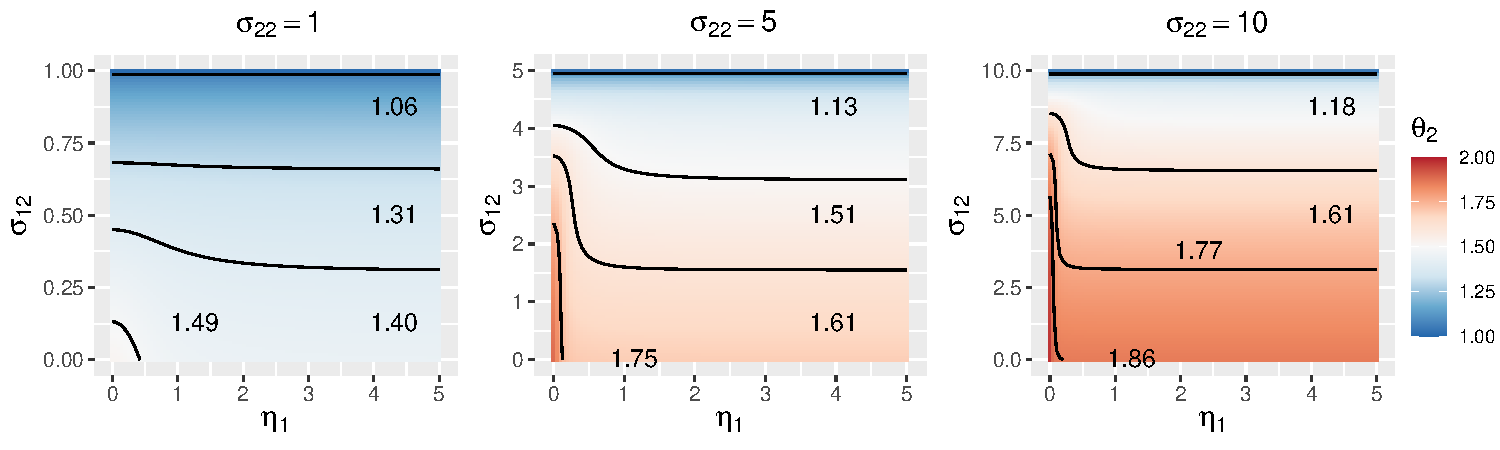
\includegraphics[width=0.95\linewidth]{bivariate_extcoef_rho_alpha.pdf}     
        \caption{}
        \label{fig:skewed_BR_extcoef}
    \end{subfigure}
    \begin{subfigure}{1\textwidth}
        \centering
        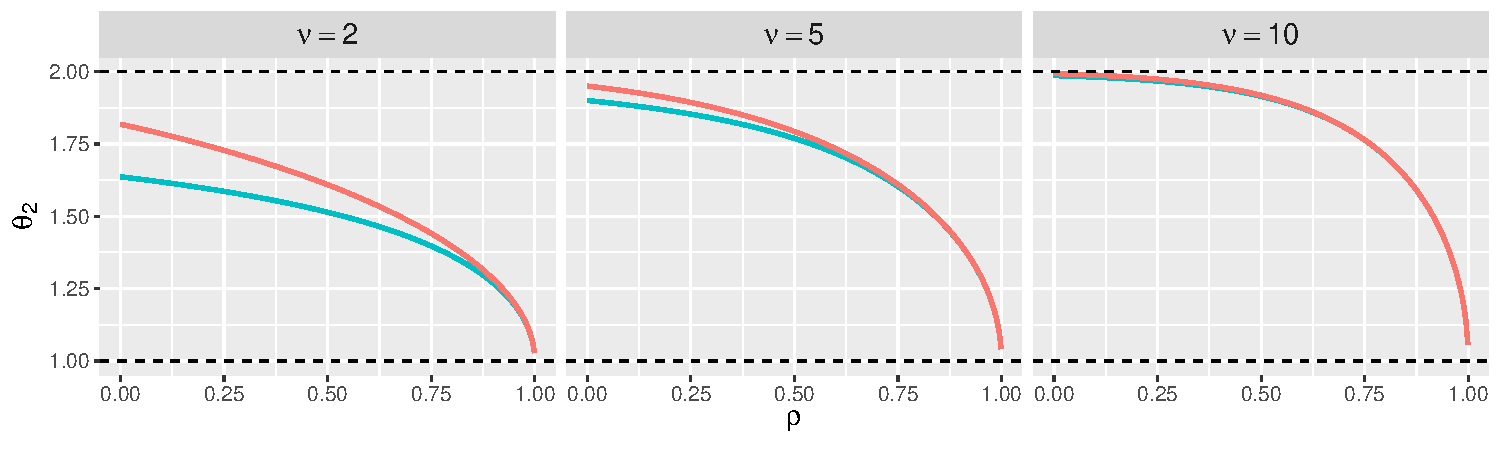
\includegraphics[width=0.95\linewidth]{bivariate_extcoef_truncT.pdf}    
        \caption{}
        \label{fig:truncated_extcoef}
    \end{subfigure}
    \caption{(a): Bivariate extremal coefficient of the skewed Brown-Resnick model ($\theta_2^{\textrm{sBR}}$) with $\bm\eta = (\eta_1,-\eta_1)^\top$ and $\Sigma = ((\sigma_{22},\sigma_{12})^\top,(\sigma_{12},\sigma_{22})^\top)$ where $\sigma_{22} = 1,5$ and $10$ (left to right), as function of $\eta_1$ and $\sigma_{12}$. (b): Bivariate extremal coefficient of the truncated extremal-t process ($\theta_2^{\textrm{tET}}$,blue) and the extremal-t process ($\theta_2^{\textrm{ET}}$, red) with $\nu=2,5$ and $10$ (left to right), as a function of the correlation parameter $\rho$.}
\end{figure}

Unlike for the Brown-Resnick, the bivariate extremal coefficient of the skewed Brown-Resnick model only partly depends on $\Sigma$ through $\gamma_{12}$, the semivariogram of the process $Y(\bs)$ defined in Theorem~\ref{thm:skewBR}. 
%
Opting for a parametrisation based on semivariogram functions over covariance functions leads to greater interpretability of the model parameters and allows for asymptotic independence in the long range when considering an unbounded variogram. Indeed, for some spatial lag $h$, taking the power-law semivariogram with range $\lambda>0$ and  smoothness $\vartheta \in (0,2]$, i.e. $\gamma(h) = (h/\lambda)^\vartheta$,
implies that, as $h \rightarrow \infty$, $\bm \eta \equiv \bm \eta (h) \rightarrow \bm 0$ and therefore $\bm \xi = \bm \xi(h) \rightarrow \bm 0$, yielding $\theta_2 \rightarrow 2$ by \eqref{eq:bi_extcoef_skewed_BR}.
%

The estimation of the $D$-dimensional parameter vector $\bm \eta$ under the constraint $\bm \eta^\top \bm 1=0$ is a difficult task that we propose to simplify by representing $\bm \eta$ through spline functions. Let $\eta_i = \sum_{j=1}^J b_{j}K_j(\bm s_i)$, $i=1, \ldots, D$, where $K_j(\bm s_i)$ is the $j$-th basis function evaluated at $\bm s_i = (s_{i,1}, s_{i,2})\in \calS$, and $b_j$ is the coefficient for the $j$-th basis. Imposing $\sum_{i=1}^D K_j(\bm s_i)=0$ automatically fulfills the sum-to-zero constraint for $\bm \eta$. 
%
In the remainder of the manuscript, $K_j(\cdot)$ denote Gaussian kernels centered at locations $\bm s_j^\star, j=1,\dots,J$, i.e.,
\begin{equation}
\label{eq:Gaussian_splines}
    K_j(\bm s_i) = \frac{K_j^\star(\bm s_i)}{\sqrt{\sum_{k=1}^D K_j^\star(\bm s_k)^2}},    
    \quad \text{where}\quad
    K_j^\star(\bm s_i) = \phi\left(\frac{\|\bm s_i-\bm s_j^\star\|}{2\sigma_B}\right)-\frac{1}{D}\sum_{k=1}^{D}\phi\left(\frac{\|\bm s_k-\bm s_j^\star\|}{2\sigma_B}\right),
    \sigma_B>0.   
\end{equation}
%
Figure~\ref{fig:skewed_BR_extcoef_spatial} displays $\theta_2^{\textrm{sBR}}$ over a $[0,32]\times[0,32]$ grid, considering $\eta_i = \sum_{j=1}^2 b_{j}K_j(\bm s_i) + 0.1\text{sgn}(s_{2,i}\geq 16)$ with $J=2$ reference points (labeled by a star), $\bm s_1^\star=(8,8)$ and $\bm s_2^\star=(24,24)$, and $\sigma_B = 64$. Note that $\text{sgn}(\cdot)$ denotes the sign function in the last term in $ \eta_i$ which serves as background noise to ensure numerical identifiability of $\bm\xi = \frac{\Sigma\bm\eta}{\sqrt{1+\bm\eta^\top\Sigma\bm\eta}}$. This is because 
%when 
multiplying $\bm\eta$ by a positive constant $c$, 
%$\bm\xi=\frac{\Sigma\bm\eta}{\sqrt{1/c^2+\bm\eta^\top\Sigma\bm\eta}}$ 
will not have a numerically significant change on $\bm\xi$ as the $\bm\eta^\top\Sigma\bm\eta$ term will dominate the denominator.
\begin{figure}[!ht]
    \centering
    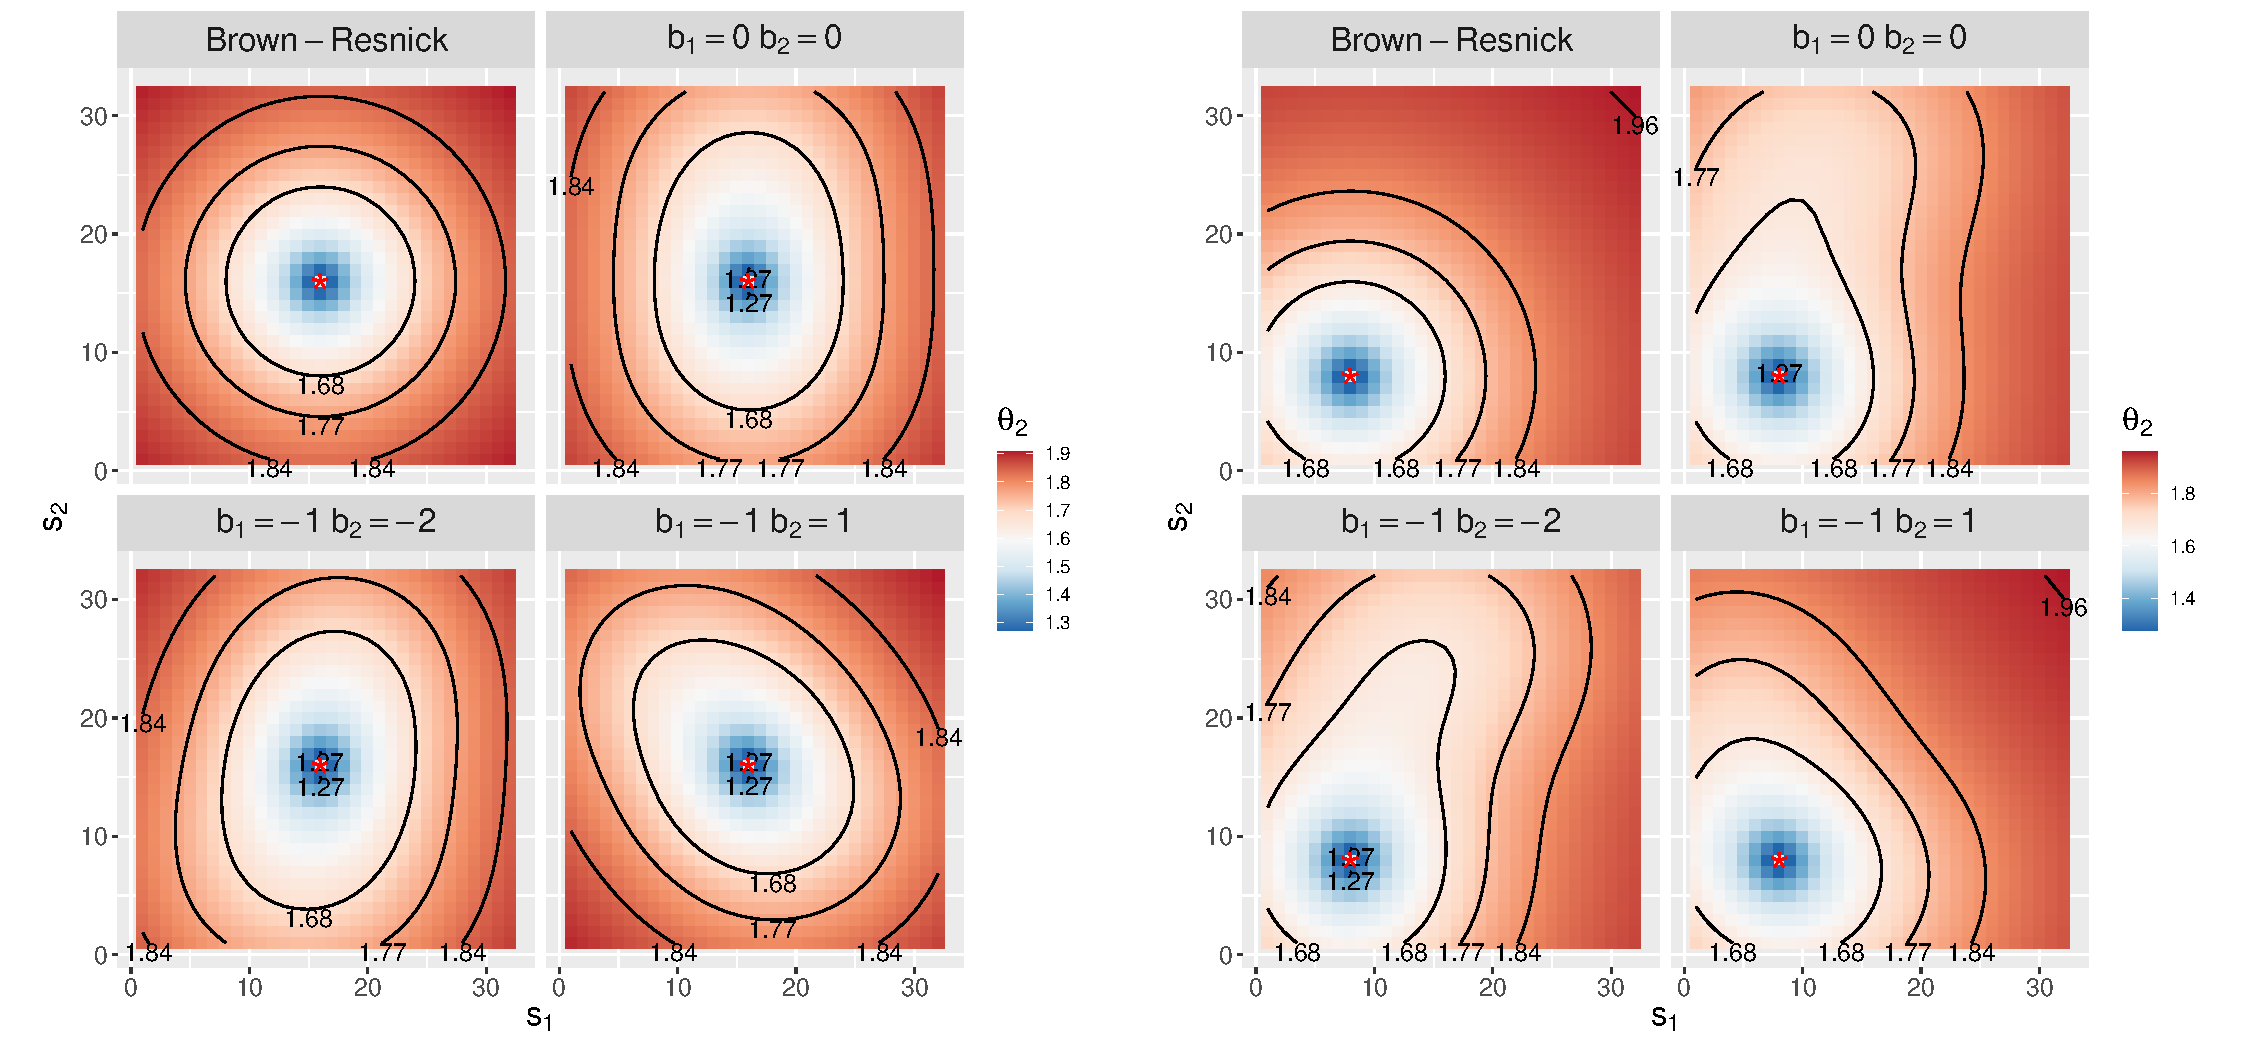
\includegraphics[width=1\textwidth]{extcoef_final_logskew.pdf}    
    \caption{Heatmaps and contour levels (solid black lines) of the bivariate extremal coefficient for the Brown-Resnick model ($\eta_i=0,i=1,\dots,D$) and skewed Brown-Resnick model where $\eta_i = \sum_{j=1}^2 b_{j}K_j(\bm s_i) + 0.1\text{sgn}(s_{2,i}\geq 16),i=1,\dots,D$ using $(b_1, b_2) = (0,0)$, $(-1,-2)$ and $(-1,-1)$. A red star indicates a different basis function reference point between left and right panels.}
    \label{fig:skewed_BR_extcoef_spatial}
\end{figure}
Focusing on a single reference point (star), i.e.~on either the four left or right panels of Figure~\ref{fig:skewed_BR_extcoef_spatial}, we observe that varying the $\bm \eta$ vector through $(b_1, b_2)$ produces a broad range of dependence structures. Similarly, for fixed parameter values $(b_1,b_2)$, different dependence behaviours are observed depending on the reference point, putting the spotlight on an important feature of the skewed Brown-Resnick process: the ability to model non-stationarity and local anisotropy. This important property, exhibited by numerous real-world environmental extreme phenomena, is due to the fact that \eqref{eq:bi_extcoef_skewed_BR} not only depends on the spatial lag between two locations, but also on the corresponding components of the $\bm \xi$ parameter vector. A similar observation was made by \citet{Beranger.etal:2017} about the extremal skew-t model.

%%%%%%%%%%%%%%%%%%%%%%%%%%%%%%%%%%%%%%%
%%%%%%%%%%%%%%%%%%%%%%%%%%%%%%%%%%%%%%%
%%%%%%%%%%%%%%%%%%%%%%%%%%%%%%%%%%%%%%%
\section{Simulation studies}
\label{sec:sim}
%%%%%%%%%%%%%%%%%%%%%%%%%%%%%%%%%%%%%%%
%%%%%%%%%%%%%%%%%%%%%%%%%%%%%%%%%%%%%%%
%%%%%%%%%%%%%%%%%%%%%%%%%%%%%%%%%%%%%%%

%%%%%%%%%%%%%%%%%%%%%%%%%%%%%%%%%%%%%%%
%%%%%%%%%%%%%%%%%%%%%%%%%%%%%%%%%%%%%%%
\subsection{Simulation algorithms}
%%%%%%%%%%%%%%%%%%%%%%%%%%%%%%%%%%%%%%%
%%%%%%%%%%%%%%%%%%%%%%%%%%%%%%%%%%%%%%%

Simulations from max-stables processes is a matured topic with algorithms developed for exact and conditional simulations. While the latter can be useful for predictions when in presence of constraints, we focus here on the former. \citet{Dombry.Engelke.Oesting:2016} proposed an approach based on the simulation of extremal functions.
%  algorithms relying on simulation from the spectral measure \citep{Dieker.Mikosch:2015} and applied for the Brown-Resnick and extremal-$t$ models. Following this approach, \citet{Beranger.etal:2021} derives the simulation algorithm for the skewed extremal-$t$. 
Following this approach, Algorithm~1 \& 2, respectively established in Section~C.4 and D.4 of the Supplementary Material, describe how to randomly generate data from the skewed Brown-Resnick and truncated extremal-$t$ models. 

Simulation algorithms for $r$-Pareto processes \citep{Dombry.Engelke.Oesting:2016,Dombry.etal:2024} involve simulations from a random vector $\bm Y$ with distribution $P_{s_i}(\cdot) = \E_{\bm W}[\mathbbm 1_{\{\bm W/W(s_i)\in \cdot\}}W(s_i)]$ at a uniformly distributed random location $s_i$, where $\bm W$ is the same as in \eqref{eq:spectralrepresentation}.
% , and such that $\bm Y/\|\bm Y\|_1$ follows the spectral distribution $\calH/D$ in \eqref{eq:decomposition} \citep[Theorem 2]{Dombry.Engelke.Oesting:2016}. 
%
This means that simulation from $r$-Pareto models can be performed by leveraging the exact simulation algorithm for max-stable models.  
%
Note that for the extremal-$t$ process, \citet[][Proposition~5]{Dombry.Engelke.Oesting:2016} shows that the random quantity $\max(\bm T,0)^\nu$, where $\bm T$ is distributed according to the multivariate Student-$t$ distribution with $\nu+1$ degrees of freedom, follows the distribution $P_{s_i}$. This makes the simulation of samples with zero values likely and therefore confirming the presence of mass on the boundaries. 

When the $L_1$ norm is selected as risk functional, i.e., $r_0(\cdot)=\|\cdot\|_1$, $r$-Pareto samples are simply obtained from $\tilde R\bm Y/\|\bm Y\|_1$, where $\tilde R$ follows a unit Pareto distribution.  
 Considering other risk functionals requires computing a constant $M$ such that $r_1 (\cdot) \leq Mr_0 (\cdot)$, where $r_1$ is another risk functional than the $L_1$ norm \citep[Proposition 2]{Dombry.etal:2024}. 
The constant $M$ is used to bound the risk functional $r_1$ from above, with the $L_1$ norm. Practically, simulation from the $r$-Pareto process with the $L_1$ norm as risk functional is first performed and rejection sampling is then applied to derive samples from the $r$-Pareto process with another risk functional, where a sample is accepted as $\bm{\tilde Z}/M$ when $r_1(\bm {\tilde Z})\geq M$. The constant $M$ takes value $D$ when $r_1$ is the infinite norm and value $D^{p-2}$ when $r_1$ is the $L_p$, $p>1$ norm.

A large constant $M$ will decrease the acceptance probability in the rejection sampling step, and thus significantly increase the computational cost of the simulation algorithm. Note that, for a risk functional $r$, the support space $\calA_r \in \mathbb R_+^D$ has complement set $\calA_r^c=\{\bm x\in\mathbb R_+^D: r(\bm x)\leq 1\}$ which is convex since $r$ is a norm and any norm defines a convex function, and we have $\calA_r\subset \calA_{r_0}$. Following from this fact, the following theorem provides an efficient simulation algorithm for $r$-Pareto processes with any convex risk functional $r$. The proof can be found in Section~E.1 of the Supplemental Material. 
%    
\begin{theorem}\label{thm:r_pareto_simulation}
Let $r$ be any risk functional that is convex, homogeneous of order 1, and such that $r(\bm 0)=0$. Suppose $r(\bm e_i)=1/c_i>0, i=1,\dots,D$, where $c_i$ are positive constants and $\bm e_i$ are the basis vector of dimension $D$, and $\bm{\tilde Z}^{(r_0)}$ is the $r$-Pareto process at $D$ locations with risk functional $r_0(\cdot)=\|\cdot\|_1$. The r-Pareto process with risk functional $r$ at $D$ locations can be then simulated as $\bm{\tilde Z}^{(r)}\eqd c_0\bm{\tilde Z}^{(r_0)}\ | \ r\left(c_0\bm{\tilde Z}^{(r_0)}\right) > 1$, where $c_0 = \min(\min_{i=1}^D c_i,1)$.
\end{theorem}
%
For example, considering $r(\cdot)=\|\cdot\|_p,\ p\in [1,\infty]$ gives $c_0 = 1$ while $r(\bm x)=\sum_{i=1}^D m_ix_i, m_i\in [0,\infty],i=1\dots,D$, (convex and homogeneous of order 1) produces $c_0=\min(\min_{i=1}^D 1/m_i,1)$. This algorithm is simpler than the one proposed by \citet{Dombry.etal:2024} since it does not require to identify the distribution for simulation.
When a risk functional, $r(\cdot)$, is not convex but only homogeneous of order 1 (e.g., $r$ returns any order statistics excluding the maximum), one can find the number $M$ such that $r (\cdot)\leq M\|\cdot\|_1$ by adopting the approach from \citet{Dombry.etal:2024}. Although this may occur, we recall that to infer about the $r$-Pareto model parameters using the score matching approach, the risk functional needs to be at least continuous and differentiable. 

In the following section, the data is randomly generated according to the algorithms derived above.

%%%%%%%%%%%%%%%%%%%%%%%%%%%%%%%%%%%%%%%
%%%%%%%%%%%%%%%%%%%%%%%%%%%%%%%%%%%%%%%
\subsection{Parameter estimation}
\label{ssec:par_est}
%%%%%%%%%%%%%%%%%%%%%%%%%%%%%%%%%%%%%%%
%%%%%%%%%%%%%%%%%%%%%%%%%%%%%%%%%%%%%%%

%%%%%%%%%%%%%%%%%%%%%%%%%%%%%%%%%%%%%%%
\subsubsection{Comparing the spectral and pairwise composite likelihoods}
%%%%%%%%%%%%%%%%%%%%%%%%%%%%%%%%%%%%%%%

In an initial experiment (see Section~F of the Supplementary Material), $500$ samples are generated from the Brown-Resnick model with large dimension ($D=225$) and, unlike the composite likelihood, the spectral likelihood produces biased estimates, especially with weaker dependence, in agreement with findings from \citet{Engelke.etal:2015, Huser.etal:2016}. Although the pairwise likelihood method is unbiased for Brown-Resnick processes, it is computationally expensive and, in this scenario, about $476$ times slower than the spectral likelihood. In addition, this approach is not available for truncated extremal-$t$ processes as the marginal distribution of a multivariate truncated normal is not a truncated normal. This necessitates a costly numerical integration for each composite likelihood term \citep{Horrace:2005}, and for skewed Brown-Resnick processes, the pairwise likelihood estimators for the skewness parameter $b_1$ and $b_2$ are found unreliable.
%
To illustrate this point, consider samples of size $n=500$ from the skewed Brown-Resnick model defined on a $15\times15$ grid with parameters $\lambda=3$, $\vartheta=1$, and $(b_1,b_2) = (-1,-2)$, where the centres of the kernels are chosen to be $\bm s_1^\star = (4,4)$ and $\bm s_2^\star=(11,11)$. 
%
The threshold for the spectral likelihood \eqref{eq:angular_likelihood_1} is set at $r_0 = 30 \times D$ and the weights in the composite likelihood \eqref{eq:composite} consider a cut-off distance to include the $1202$ closest pairs to mitigate the computational complexity.
% 
After replicating the estimation procedure $300$ times (as for all upcoming experiments), violin plots of the estimators are displayed in Figure~\ref{fig:simulation_boxplot_skewedBR_comp}, showcasing almost unbiased estimates for $b_1$ and $b_2$ and small relative bias (around $10\%$) for $\lambda$ and $\vartheta$ when the spectral likelihood (red) is applied. 
%
In contrast, the pairwise likelihood estimates (blue) for $\lambda$ and $\nu$ are unbiased, but those for $b_1$ and $b_2$ are biased and almost unreliable, which may be attributed to the inability of this approach to capture the locally anisotropic dependence structure presented in the data. The spectral likelihood is about $68$ times faster than the composite likelihood, taking $124$ seconds on a $16$-core machine and considering multiple initial values for the skewness parameter to avoid local maxima.  
%
\begin{figure}[!ht]
    \centering
    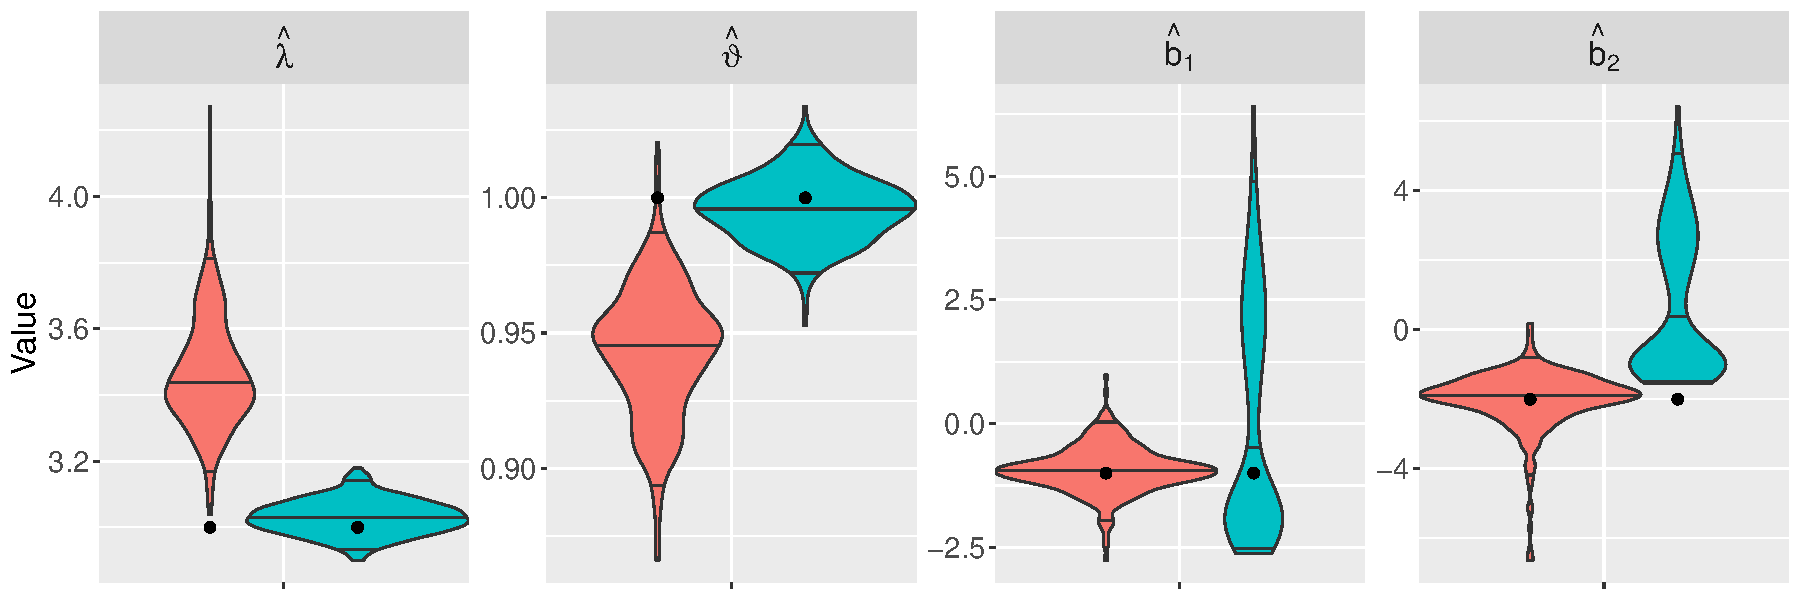
\includegraphics[width=0.95\textwidth]{simulation_est_boxplots_final_skewBR_comp.pdf}
    \caption{Violin plots for 300 estimates of $\bm \theta = (\lambda, \vartheta, b_1, b_2)$ for the skewed Brown-Resnick process with $\lambda=3$, $\vartheta=1$, and $(b_1,b_2) = (-1,-2)$ using the spectral likelihood (red) with threshold $T=30\times D$ and the pairwise likelihood (blue) with 1202 pairs. Black dots indicate the true values.}
    \label{fig:simulation_boxplot_skewedBR_comp}
\end{figure}
%   

%%%%%%%%%%%%%%%%%%%%%%%%%%%%%%%%%%%%%%%
\subsubsection{Impact of the threshold selection in the spectral likelihood}
%%%%%%%%%%%%%%%%%%%%%%%%%%%%%%%%%%%%%%%

When interested in fitting a spatial extremes model through the spectral likelihood, a natural question is: what is a good choice of threshold value $r_0$? While the answer is not trivial, some insights can be drawn by the following two experiments.

First, we focus again on the skewed Brown-Resnick model but increase the sample size to $2000$ and consider 12 parameter combinations with $\lambda=5,10$, $\vartheta = 1,1.5$, and $(b_1,b_2) = (0,0),(-1,-2),(-1,1)$. The grid size and centres of the kernels remain unchanged. The spectral likelihood is fitted where the threshold is increased to $r_0=100\times D$, retaining approximately the $20$ observations with largest radial component. Violin plots for each parameter estimate and true parameter combination (indicated as case $1-12$) provided in Figure~\ref{fig:simulation_boxplot_skewedBR} highlight the ability to accurately identify all parameters, no matter the degree of dependence. This confirms that, even with roughly the same number of observations, increasing $r_0$ reduces the bias in the spectral likelihood since the Poisson approximation is better. Finally, note that model fitting is computationally efficient, taking on average about $6$ minutes using 16 cores and setting multiple initial values for the skewness parameter.
%
\begin{figure}[!ht]
    \centering
    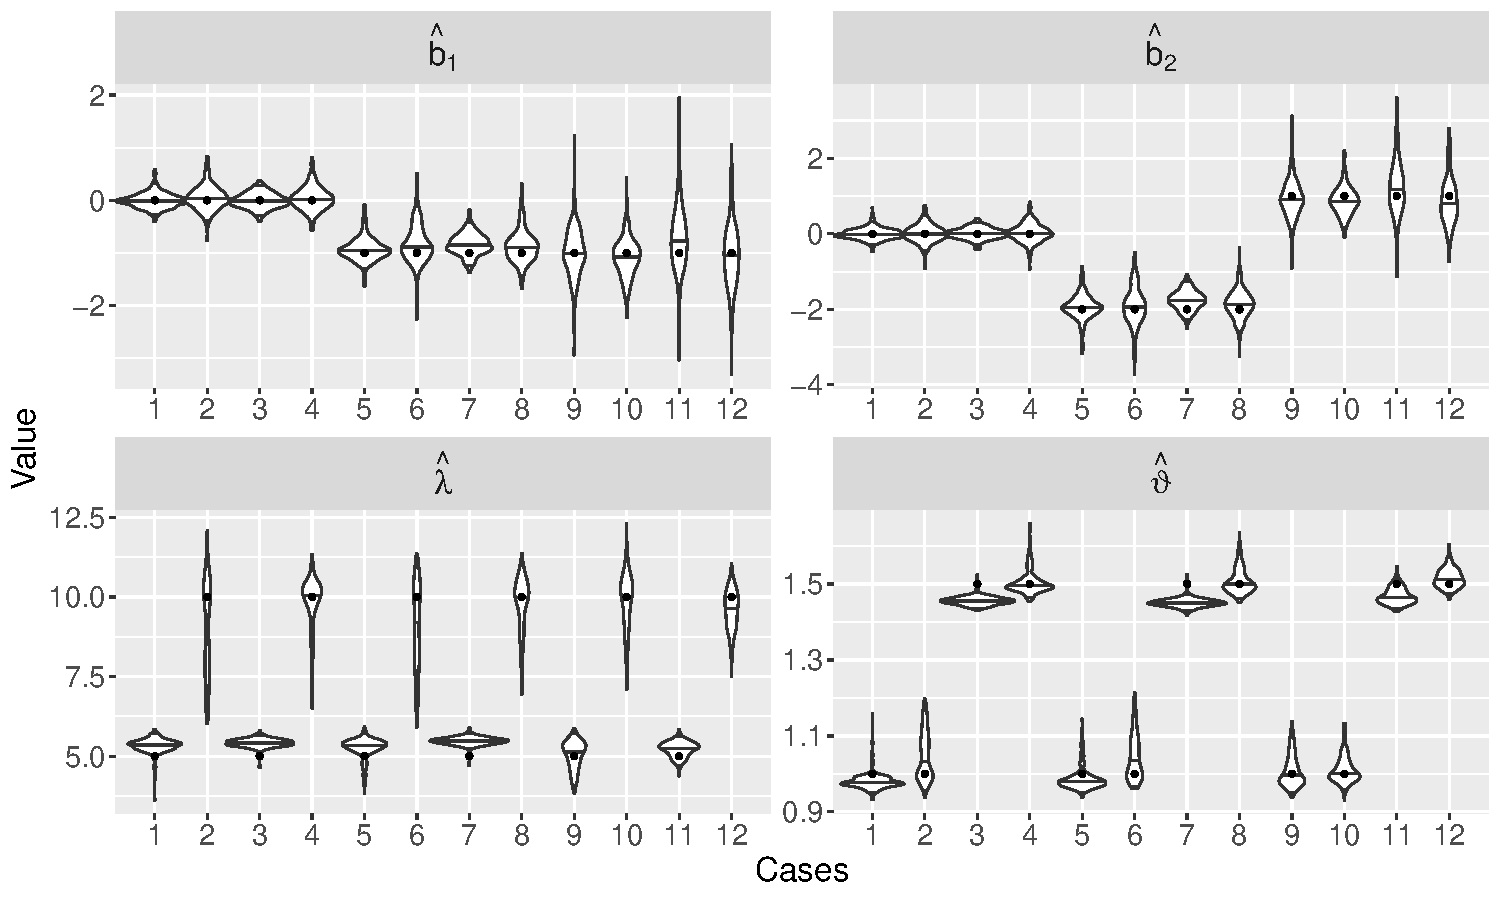
\includegraphics[width=0.95\textwidth]{simulation_est_boxplots_final.pdf}    
    \caption{Violin plots for the 300 estimates of $\bm \theta= \left(\lambda, \vartheta,  b_1, b_2\right)$ for the skewed Brown-Resnick process with $\lambda=5,10$, $\vartheta=1,1.5$, and $(b_1,b_2) = (0,0),(-1,-2),(-1,1)$, using the spectral likelihood. Black dots indicate the true values.}
    \label{fig:simulation_boxplot_skewedBR}
\end{figure}
%

Next, we shift our focus on the truncated extremal-$t$ model on a $10\times10$ grid ($D=100$) where $2000$ samples are generated from 2 parameter combinations using $\lambda=3, 5$, $\vartheta=1$ and $\nu=2$.
%
The spectral likelihood is again fitted where the degree of freedom is fixed to its true value ($\nu=2$). Figure~\ref{fig:simulation_boxplot_truncT} displays violin plots of the estimates $\hat{\lambda}$ and $\hat{\vartheta}$ when the threshold $r_0$ set as the $98\%$ (red), $95\%$ (green), and $90\%$ (blue) quantiles of the observed radial components.
%
For a sample size $n=2000$, retaining the $40$ ($r_0=98\%$) observations with the largest radial components produces almost unbiased estimates. Lowering $r_0$ increases the bias but also increases the computation time since more observations are included. As highlighted in Section~\ref{ssec:new_models}, fitting the truncated extremal-$t$ model requires more computational effort than the skewed Brown-Resnick, here taking on average about 15 minutes.   
%
Overall, the practical recommendation is to select a threshold as high as possible while ensuring that enough observations are kept in order to control the variability of the estimates.
%
\begin{figure}[!ht]
    \centering
    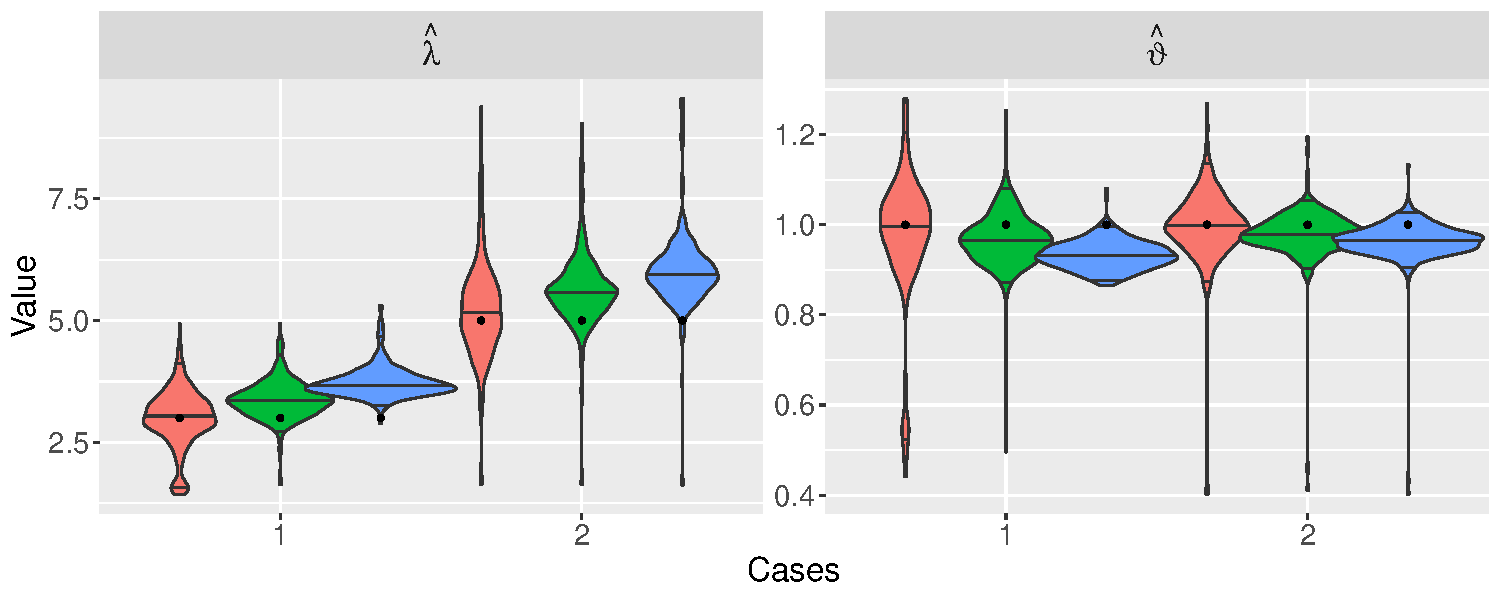
\includegraphics[width=0.95\textwidth]{simulation_est_boxplots_final_truncT.pdf}    
    \caption{Violin plots for the spectral likelihood estimates of the truncated extremal-$t$ model with $\lambda=3,5$, $\vartheta=1$, and $\nu=2$ (fixed), and threshold $r_0$ set as the $98\%$ (red), $95\%$ (green) and $90\%$ (blue) empirical quantiles of the radial component. Black dots indicate the true parameter values.}
    \label{fig:simulation_boxplot_truncT}
\end{figure}
%

%%%%%%%%%%%%%%%%%%%%%%%%%%%%%%%%%%%%%%%
\subsubsection{Comparing the spectral likelihood and score matching approach}
%%%%%%%%%%%%%%%%%%%%%%%%%%%%%%%%%%%%%%%

The interest is now in fitting $r$-Pareto processes with different risk functionals and investigating the performance of the spectral likelihood over the well-adopted score matching approach \citep[see][]{deFondeville.Davison:2018}. 
%
We sample $2000$ observations from the skewed Brown-Resnick $r$-Pareto process defined on a $15\times15$ grid with the same parameter combinations as in Figure~\ref{fig:simulation_boxplot_skewedBR}. Taking the $L_1$ and $L_3$ norms as risk functionals, an observation is considered extreme when exceeding the threshold $u$ which selected as the $95\%$ empirical quantile of $r(\bm X_1),\dots,r(\bm X_n)$.

Estimation outputs when the risk functional is the $L_3$ norm are given as violin plots in Figure~\ref{fig:simulation_boxplot_rpareto_skewedBR} for $\hat{\vartheta}$ and $\hat{b}_1$. For completeness, equivalent plots for $\hat{\lambda}$ and $\hat{b}_2$ are reported in Figure~2, Section~E.3 of  the Supplementary material.
%
Across all dependence structure regimes, the spectral likelihood consistently provides estimates (blue) for all four parameters that are unbiased and with small variability. On the contrary, although the score matching approach is able to produce unbiased but more variable estimates (red) of $\lambda$ and $\vartheta$, it becomes numerically unstable for the skewness parameters, in particular for cases $7-12$.
% 
On top of being more statistically efficient, the spectral likelihood is also more computationally efficient since it is about $5$ times faster than the score matching approach (141 versus 704 seconds on average using 3 CPU cores). 
%
Similar results and conclusions can be drawn when the risk functional is the $L_1$ norm and therefore reported in Figure~3 of the Supplementary Material.
%
% \begin{figure}[ht]
%     \centering
%     \includegraphics[width=1\textwidth,page=2]{simulation_pareto_violin__5_Inf_Inf.pdf}    
%     \caption{Violin plots for the score matching (left) and spectral likelihood (right) estimates of $\bm \theta= \left(\lambda, \vartheta,  b_1, b_2\right)$ for the skewed Brown-Resnick $r$-Pareto process with $L_3$ norm risk functional and the same parameter combinations as in Figure~\ref{fig:simulation_boxplot_skewedBR}. Black dots indicate the parameter true values. \textcolor{red}{Need to improve the quality of those plots.}}
%     \label{fig:simulation_boxplot_rpareto_skewedBR}
% \end{figure}
\begin{figure}[ht]
    \centering
    \includegraphics[width=0.95\textwidth,page=6]{simulation_pareto_violin_logskew_5.pdf}
    \includegraphics[width=0.95\textwidth,page=7]{simulation_pareto_violin_logskew_5.pdf}
    \caption{Violin plots for the score matching (red) and spectral likelihood (blue) estimates of $\vartheta$ (top) and  $b_1$ (bottom) for the skewed Brown-Resnick $r$-Pareto process with $L_3$ norm risk functional and the same parameter combinations as in Figure~\ref{fig:simulation_boxplot_skewedBR}. Black dots indicate the parameter true values.}
    \label{fig:simulation_boxplot_rpareto_skewedBR}
\end{figure}
%
For completeness, experiments on the truncated extremal-$t$ $r$-Pareto process are also conducted on a $8\times8$ grid with $8$ parameter combinations, and presented in Figure~4 of the Supplementary Material.

In conclusion, the above experiments indicate that the spectral likelihood is a statistically and computationally efficient methodology that can infer the model parameters of max-stable and $r$-Pareto processes, an in particular the newly introduced skewed Brown-Resnick and truncated extremal-$t$ models. For max-stable processes, a carefully selected threshold $r_0$ will allow to control the bias in the estimates due to the Poisson approximation while for $r$-Pareto processes this approximation no longer exist and the method provide unbiased estimates with small variance. The computational gains are significant and allow to tackle higher dimensional problems.

%%%%%%%%%%%%%%%%%%%%%%%%%%%%%%%%%%%%%%%
%%%%%%%%%%%%%%%%%%%%%%%%%%%%%%%%%%%%%%%
%%%%%%%%%%%%%%%%%%%%%%%%%%%%%%%%%%%%%%%
\section{Real-world applications}
\label{sec:real}
%%%%%%%%%%%%%%%%%%%%%%%%%%%%%%%%%%%%%%%
%%%%%%%%%%%%%%%%%%%%%%%%%%%%%%%%%%%%%%%
%%%%%%%%%%%%%%%%%%%%%%%%%%%%%%%%%%%%%%%

%%%%%%%%%%%%%%%%%%%%%%%%%%%%%%%%%%%%%%%
%%%%%%%%%%%%%%%%%%%%%%%%%%%%%%%%%%%%%%%
\subsection{Analysis of extreme rainfall over Florida}
%%%%%%%%%%%%%%%%%%%%%%%%%%%%%%%%%%%%%%%
%%%%%%%%%%%%%%%%%%%%%%%%%%%%%%%%%%%%%%%

The spatial dependence structure of rainfall across the Tampa Bay area, Florida, during the wet season (June--September) is investigated. The data consists of radar measurements recorded at 15 minute intervals between 1995 and 2019, over a regular 2km grid. The dataset is made of $n=139,881$ radar images with $4,449$ spatial observations in each image.
%
\cite{deFondeville.Davison:2018} fitted a $r$-Pareto process based on Brown-Resnick model to a subset of this data restricted to the 1999 to 2004 period and $3,600$ locations. 
%
The same fitting procedure is applied here as a benchmark to demonstrate the advantages of using the spectral likelihood. In addition, to further motivate the need for a broader class of models, the skewed Brown-Resnick model is fitted with spline representation of $\bm\eta$ as in Section~\ref{ssec:flex_dep} with four kernels (see black dots in Figure~\ref{fig:extcoef_application_florida}).
%
In a first step, the data are marginally transformed to unit Pareto scale using the empirical distribution function, while zero values are ignored and treated as missing. 
%
An anisotropic semivariogram function is adopted, i.e.,
%
\begin{equation*}
    \gamma(\bm h) = \left(\frac{\left\| V \bm h\right\|_2}{\lambda}\right)^\vartheta, \vartheta\in(0,2],\lambda>0,
\end{equation*}
%
where $\bm h$ is the difference vector between coordinates of two locations and $V$ is a matrix used to capture the global anisotropy in the dependence structure given by
%
\begin{equation}
\label{eq:aniso_mat}
    V = \begin{pmatrix}
    \cos\zeta & - \sin\zeta\\
    m\sin\zeta &  m\cos\zeta
    \end{pmatrix}, m >0 , \zeta\in (-\frac{\pi}{4},\frac{\pi}{4}).
\end{equation}
%
The $r$-Pareto processes are defined using the $L_1$ and $L_\infty$ norms as the risk functionals. These choices are motivated by the fact that the $L_\infty$ norm defines extremes events as locally intense rainfall events at any location within the region, whereas the $L_1$ norm selects events with high cumulative rainfall over the whole region. Although these types of events are of different nature, both can lead to flooding and both have recently occurred in Florida. For example, a plume of moisture caused heavy rainfall in southern Florida on June 11, 2024 generating high risks of localised flash flooding whereas hurricanes Irma and Milton (September 2017 and October 2024) lasted several days and touched large parts of the state. 
%
To choose the thresholds, a univariate generalized Pareto distribution is fitted to the values of the corresponding risk functional evaluated at each observations and the level for which the estimated shape parameter becomes stable is selected. 
%
As a result, the threshold $u$ is set as the $99.95\%$ empirical quantile of $r(\bm X_1),\dots,r(\bm X_n)$ for both $L_1$ and $L_\infty$ norm risk functionals, leaving the $70$ most extreme observations for model fitting. 
%
% Averaging the computation times for both risk functions, the skewed Brown-Resnick and Brown-Resnick $r$-Pareto models are fitted using the spectral likelihood in about 8.00 and 0.85 hours respectively, with a 16-core machine. Such difference in computing time is simply due to the model complexity, the skewed Brown-Resnick having an additional $4$ parameters.
% 

Table~\ref{tab:parameter_estimates} reports the parameter estimates (with jackknife estimates of the standard errors in parentheses) for both models (denoted as sBR and BR) and risk functional ($L_1$ and $L_\infty$). Note that inference was performed on a 16-core machine and for interpretability, the estimates of the range parameter are given in km unit.
%
Inferring about the Brown-Resnick parameters using either the spectral likelihood or the score matching method (respectively denoted by BR and $\textrm{BR}^*$) results in estimates within the same range, no matter the risk functional (perhaps to the exception of $\lambda$). Supporting the conclusions from the simulation experiments, the spectral likelihood approach is respectively $80\%$ and $18\%$ faster than the score matching when selecting $L_1$ and $L_\infty$ risk functionals. 
%
Inference for the skewed Brown-Resnick (sBR) is much slower, taking several hours, which reflects the presence of $4$ additional parameters. All computation reported in this section and the next one are performed on a 16-core machine.

Now comparing the model fits obtained from the spectral likelihood, both outputs indicate no evidence against the parameter $m$ taking value one implying that there is no global anisotropy in the dependence structure, a finding consistent with \cite{deFondeville.Davison:2018}. 
%
The standard errors of the slant parameters $b_1$--$b_4$ are relatively large and although confidence intervals would include zero, it cannot be concluded that there is no evidence these parameters are different from zero. Indeed, unlike in the simulation experiments, no background noise has been added in the representation of the $\bm \eta$ parameter and therefore identifiability issues are reflected in the jackknife estimates of the standard errors.
%
The greater flexibility in the dependence structure of the skewed Brown-Resnick is however demonstrated by lower values of the Akaike Information Criterion (AIC) when considering either risk function (respectively $2482.39$ against $2485.88$ and $2510.44$ against $2526.61$). Preference for the skewed Brown-Resnick model indicates that a local anisotropic dependence structure is detected.

%
Figure~\ref{fig:extcoef_application_florida} provides a map of empirical bivariate extremal coefficients with respect to two different reference points which is used to assess the goodness-of-fit of the skewed Brown-Resnick and Brown-Resnick models respectively represented by solid and dashed contour lines for 8 levels (1.2,1.5,1.7,1.75,1.8,1.85,1.9, and 1.95). Across all panels, the contours from the skewed Brown-Resnick model seem to be able to pick up the directional anisotropic pattern exhibited by the empirical estimates. 
% The higher values along the North-South axis are indeed consistent with the anisotropy matrix used in the model. 
Furthermore, the patterns of the empirical extremal coefficient appear to vary with the reference location, a property unique to the skewed Brown-Resnick model.
%
Comparing the insights drawn between risk functionals, the $L_\infty$ norm seems to lead to a localised extremal dependence structure, whereas the $L_1$ norm produces a dependence that is more persistent with distance. These remarks are coherent with the interpretation of the extreme events selected by these risk functional ($L_1$ norm  = cumulative rainfall over the whole region; $L_\infty$ norm  = location-wise rainfall). 
%
For completeness, Figure~5 of the Supplementary material displays the extremal coefficients of the Brown-Resnick model for both inference approaches indicating the estimate of the range parameter $\lambda$ obtained using score matching is likely underestimated. 
%
\begin{table}[!ht]
    \centering
    \scalebox{0.8}{
        \begin{tabular}{lccccccccccc}
            \hline
           Model & $r(\cdot)$ & $\hat\lambda$ & $\hat\vartheta$ & $\hat\zeta$ & $\hat m$ & $\hat b_1$ & $\hat b_2$ & $\hat b_3$ & $\hat b_4$ & \textrm{Time (hrs)}\\ 
            \hline                
            $\textrm{BR}^*$ & $L_1$ & 2.80 & 1.40 & -0.12 & 1.06 & - & - & - & - & 2.05\\ 
              & & (0.25) & (0.09) & (1.25) & (0.07) & - & - & - & - \\
            BR & $L_1$ & 5.91 & 1.16 & -0.73 & 0.96 & - & - & - & - & 1.14\\ 
              & & (1.71) & (0.11) & (1.21) & (0.07) & - & - & - & - \\ 
            $\textrm{BR}^*$ & $L_\infty$ & 3.49 & 1.71 & -0.04 & 1.02 & - & - & - & - & 1.90 \\ 
              & & (0.22) & (0.04) & (1.83) & (0.05) & - & - & - & - \\   
            BR & $L_\infty$ & 6.30 & 1.37 & 0.40 & 0.95 & - & - & - & - & 1.70 \\ 
              & & (0.39) & (0.03) & (0.36) & (0.04) & - & - & - & - \\ 
            sBR & $L_1$ & 5.81 & 1.19 & 0.73 & 1.04 & 11.39 & 8.58 & 23.09 & 19.89 & 4.20 \\ 
              & & (1.74) & (0.11) & (2.83) & (0.15) & (27.15) & (21.37) & (56.21) & (47.90) \\ 
            sBR & $L_\infty$ & 5.96 & 1.41 & 0.46 & 0.96 & 0.16 & 0.15 & 0.06 & 0.07 & 4.94 \\ 
              & & (0.35) & (0.03) & (0.28) & (0.04) & (1.22) & (1.22) & (0.52) & (0.48) \\ 
            \hline
        \end{tabular}
    }
    \caption{Parameter estimates (jackknife estimates of the standard errors) for the Brown-Resnick (BR) and skewed Brown-Resnick (sBR) $r$-Pareto models $L_1$ and $L_\infty$ norm risk functional. Model name with an asterisk ($^*$) indicate inference was performed using the score matching approach.}
    \label{tab:parameter_estimates}
\end{table}
%
\begin{figure}[!ht]
    \centering
    \begin{subfigure}{0.45\textwidth}
        \centering
        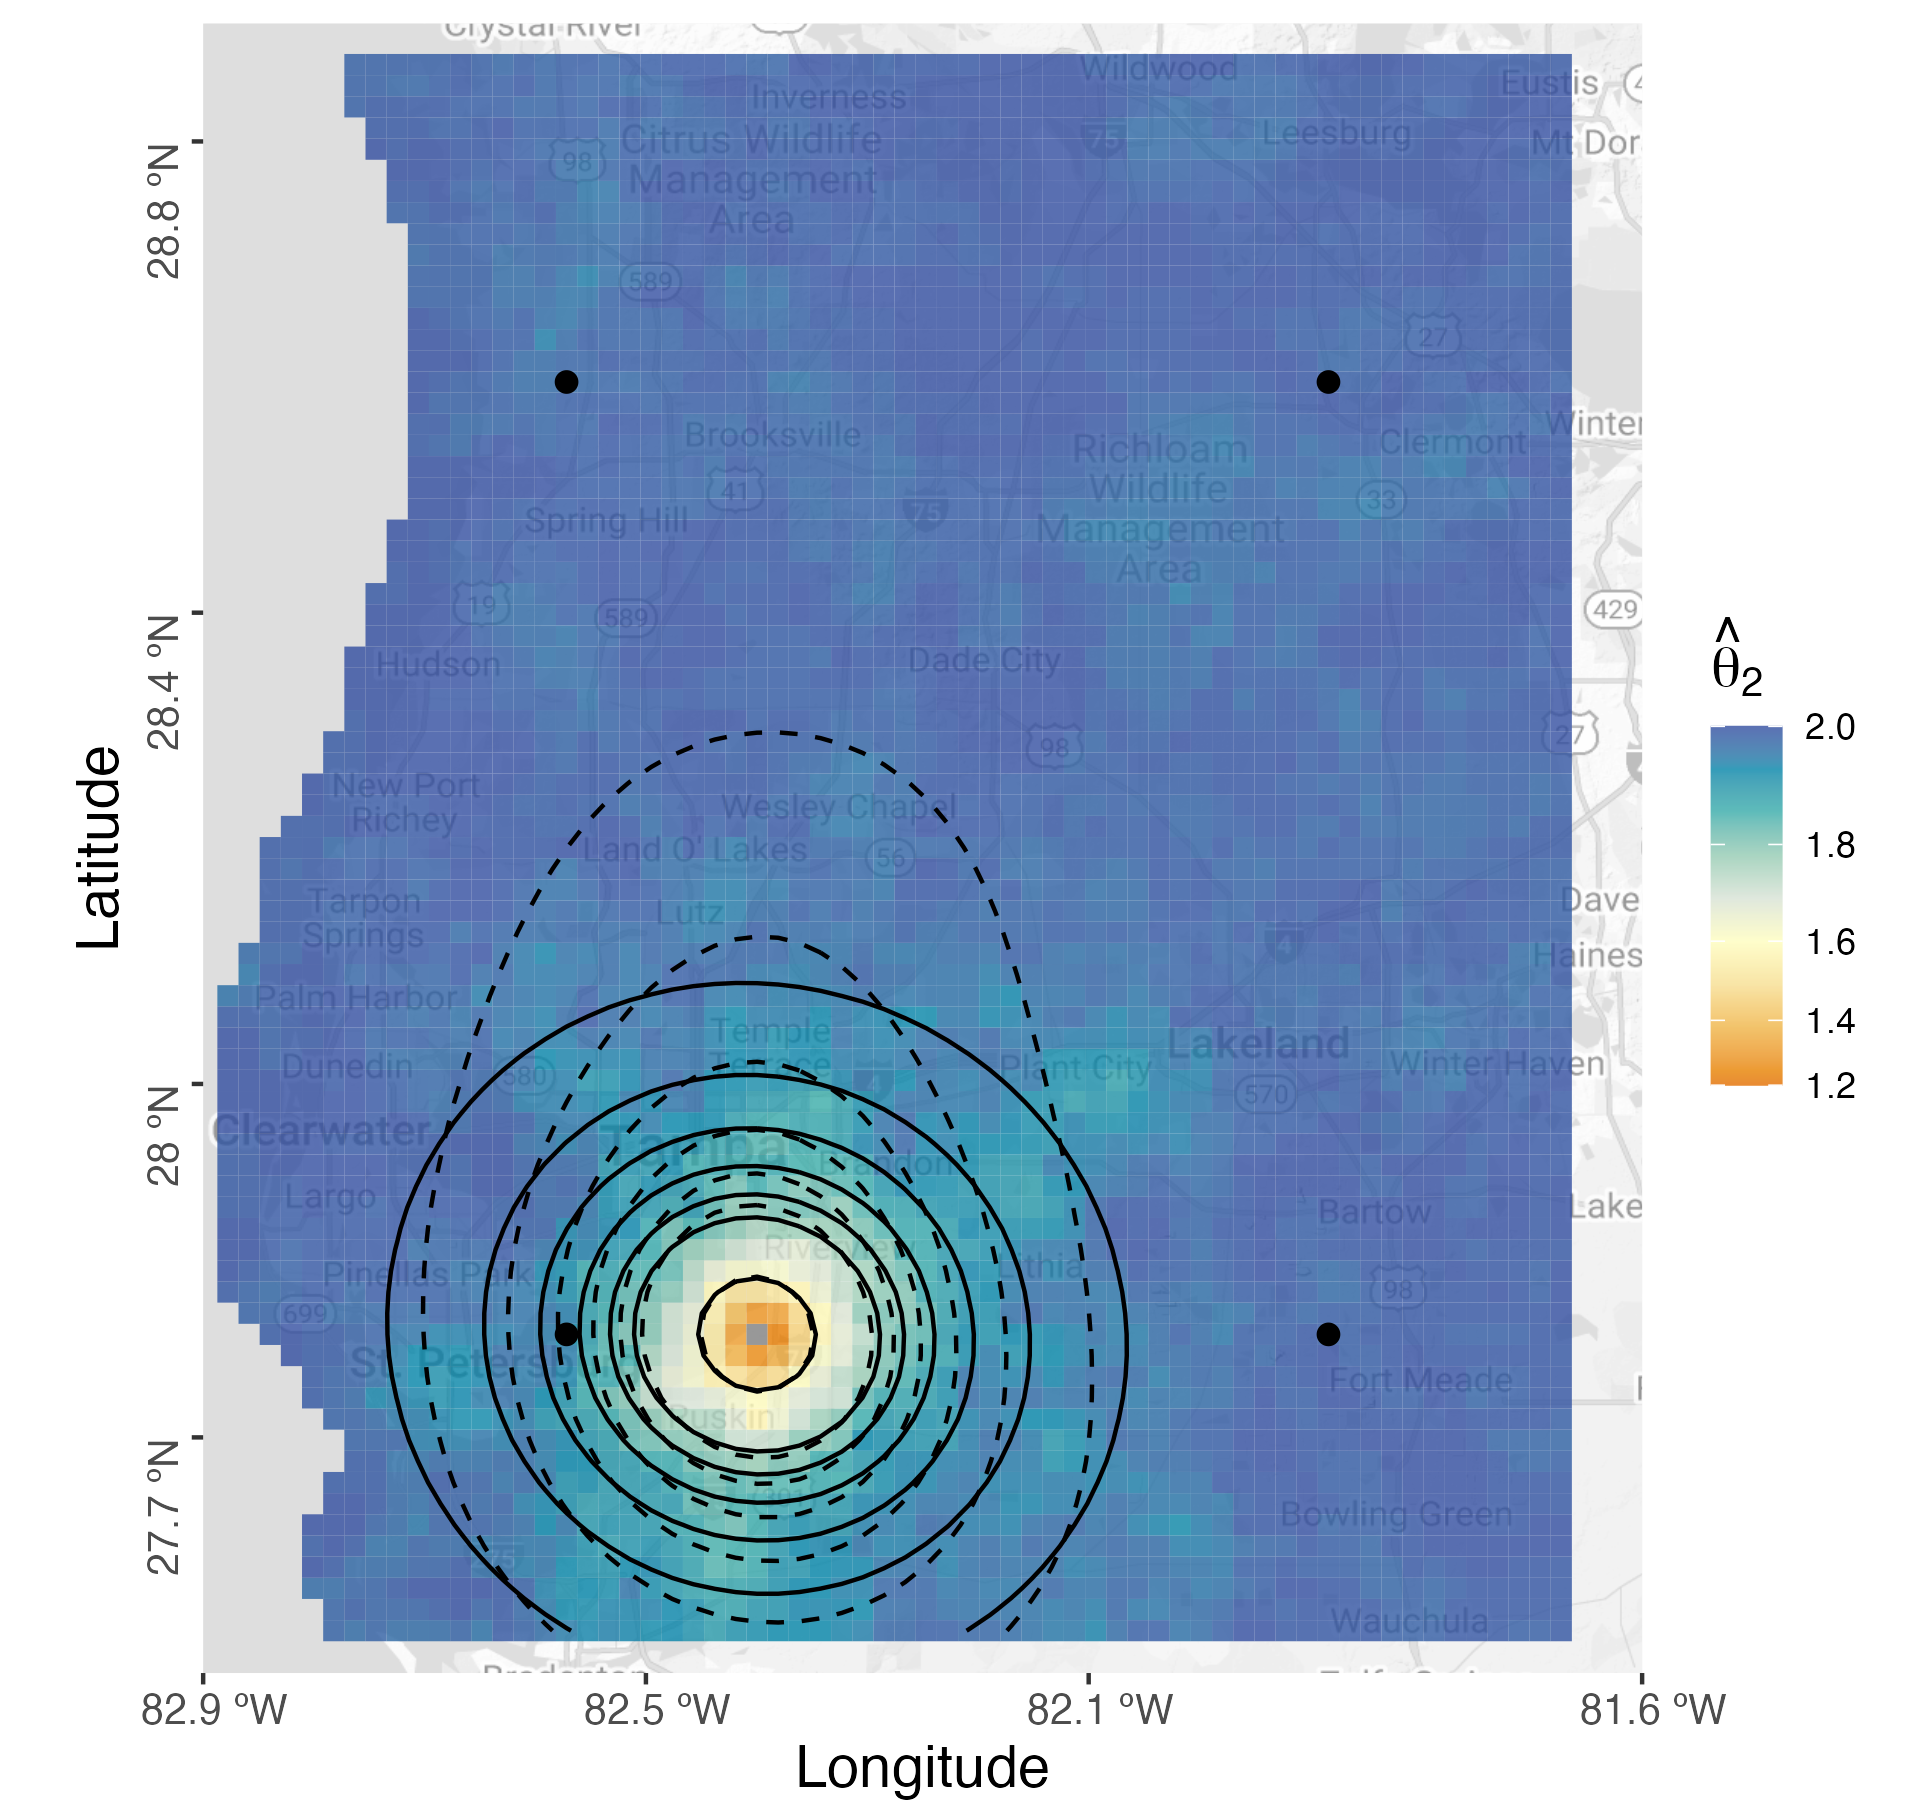
\includegraphics[width=1\textwidth]{florida/florida_extcoef2_1_008.png}
    \end{subfigure}%
    \begin{subfigure}{0.45\textwidth}
        \centering
        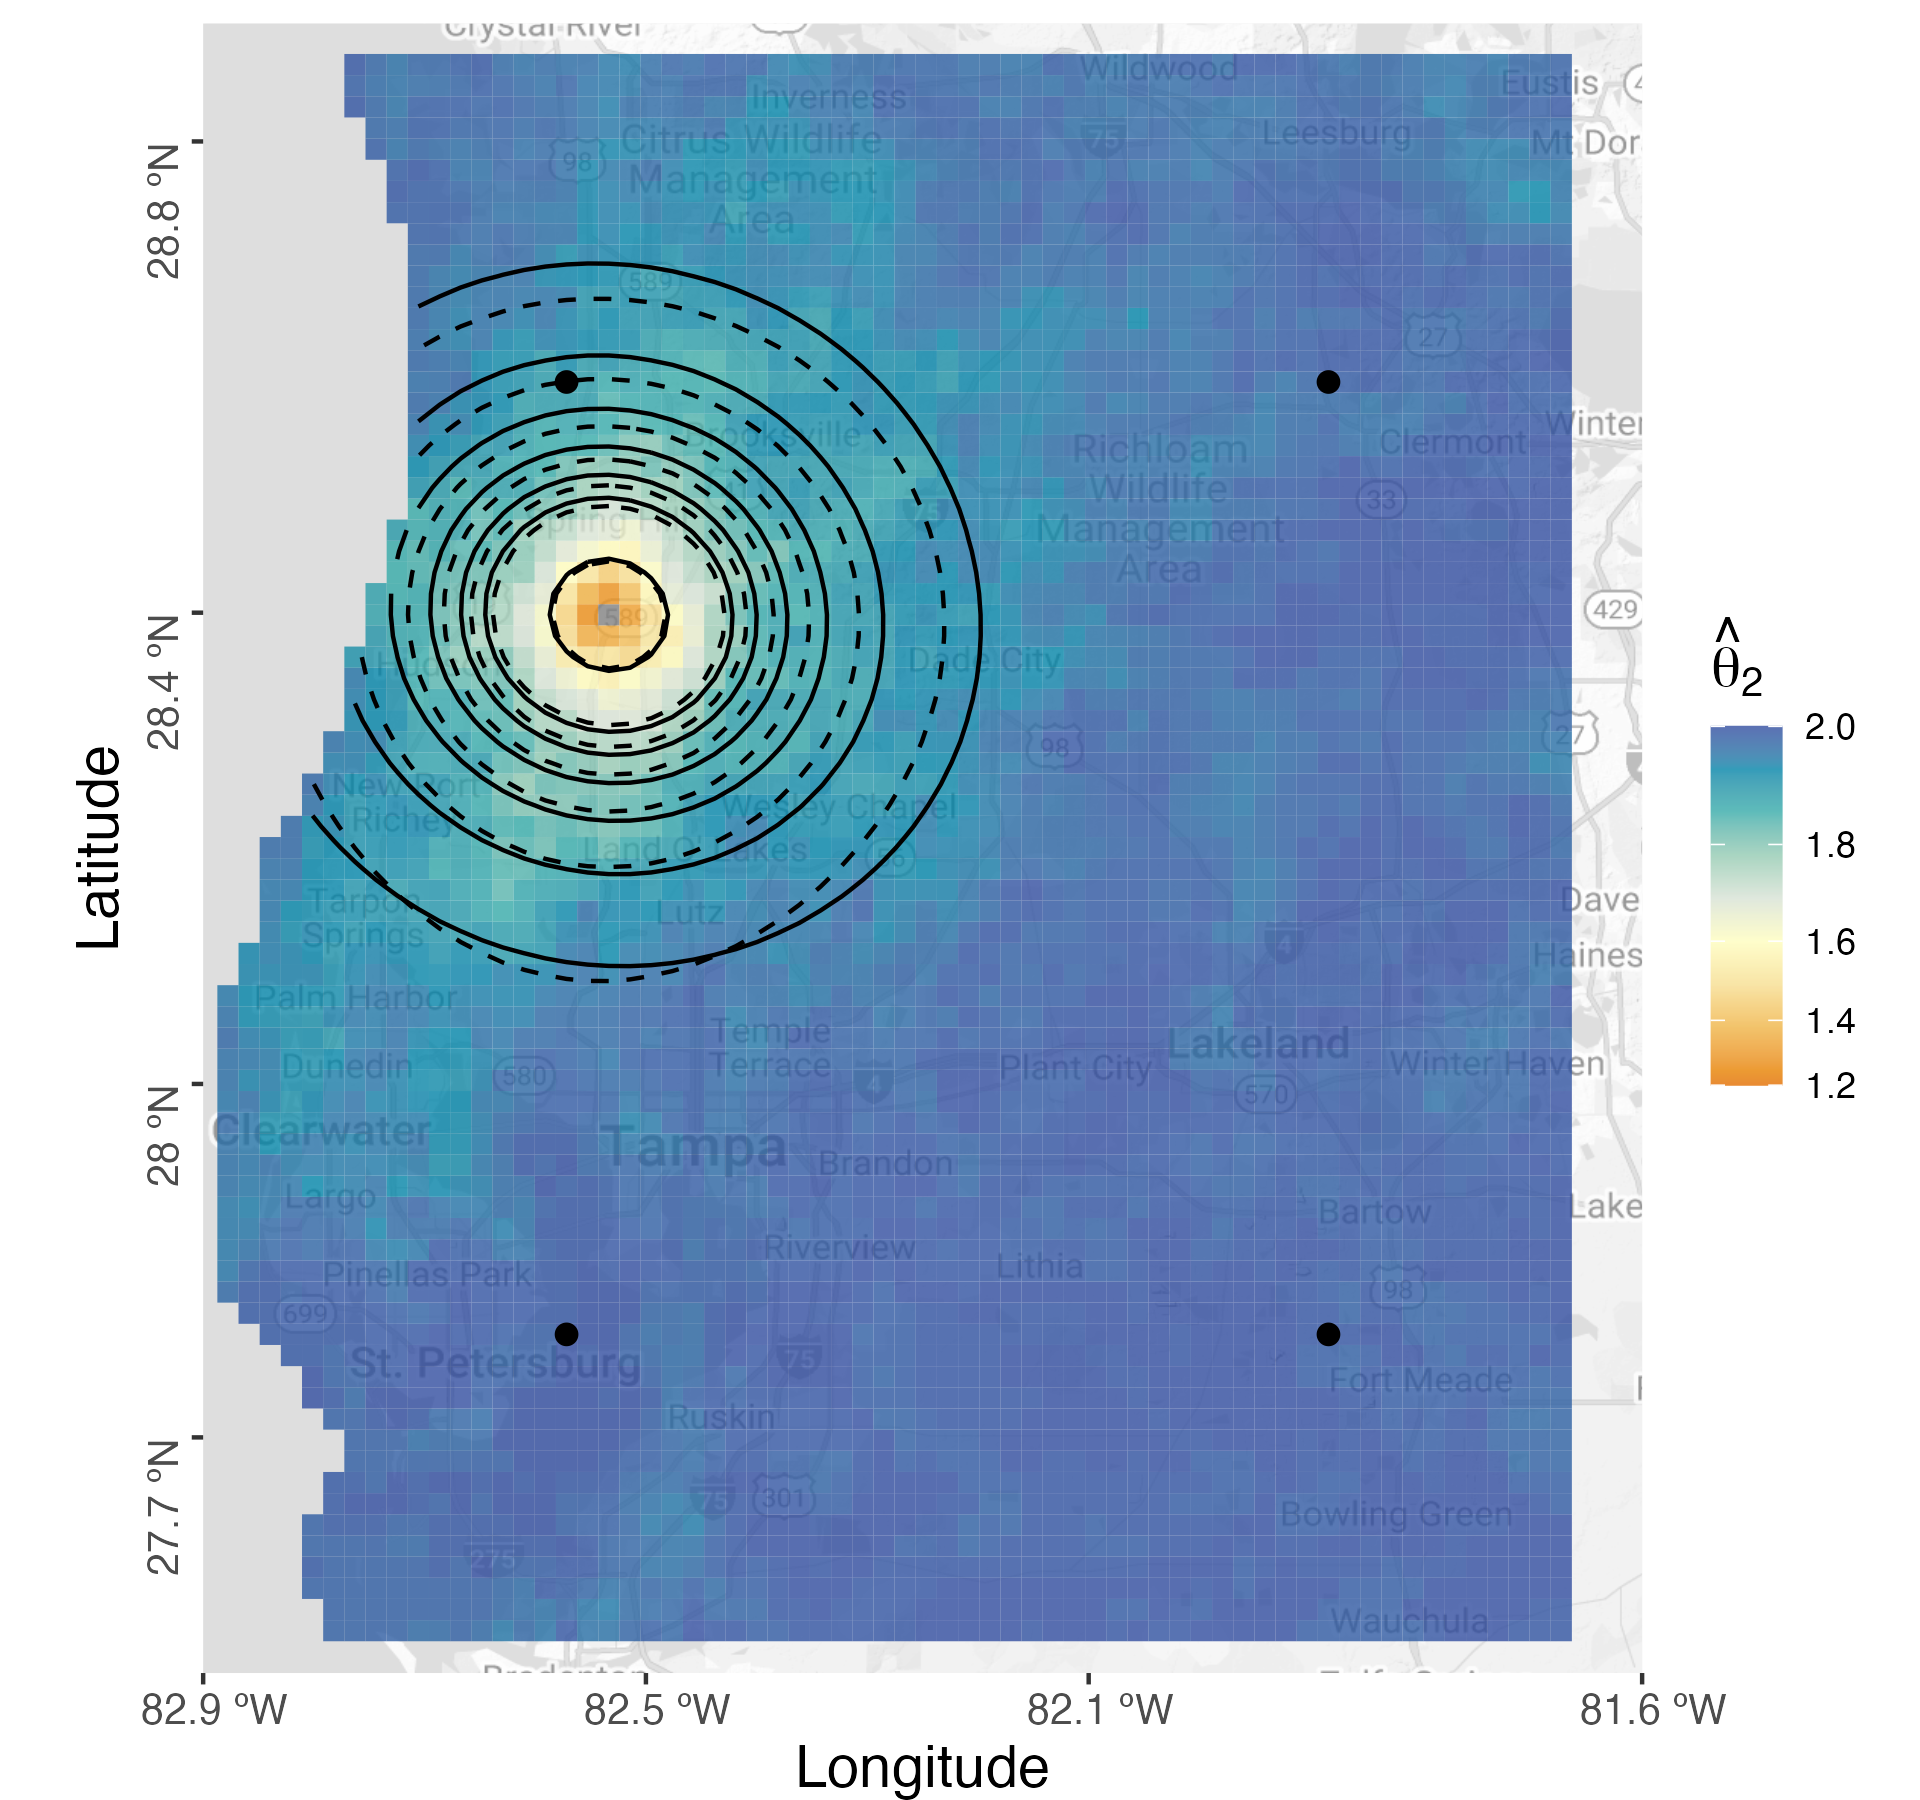
\includegraphics[width=1\textwidth]{florida/florida_extcoef2_1_038.png}
    \end{subfigure}
    \begin{subfigure}{0.45\textwidth}
        \centering
        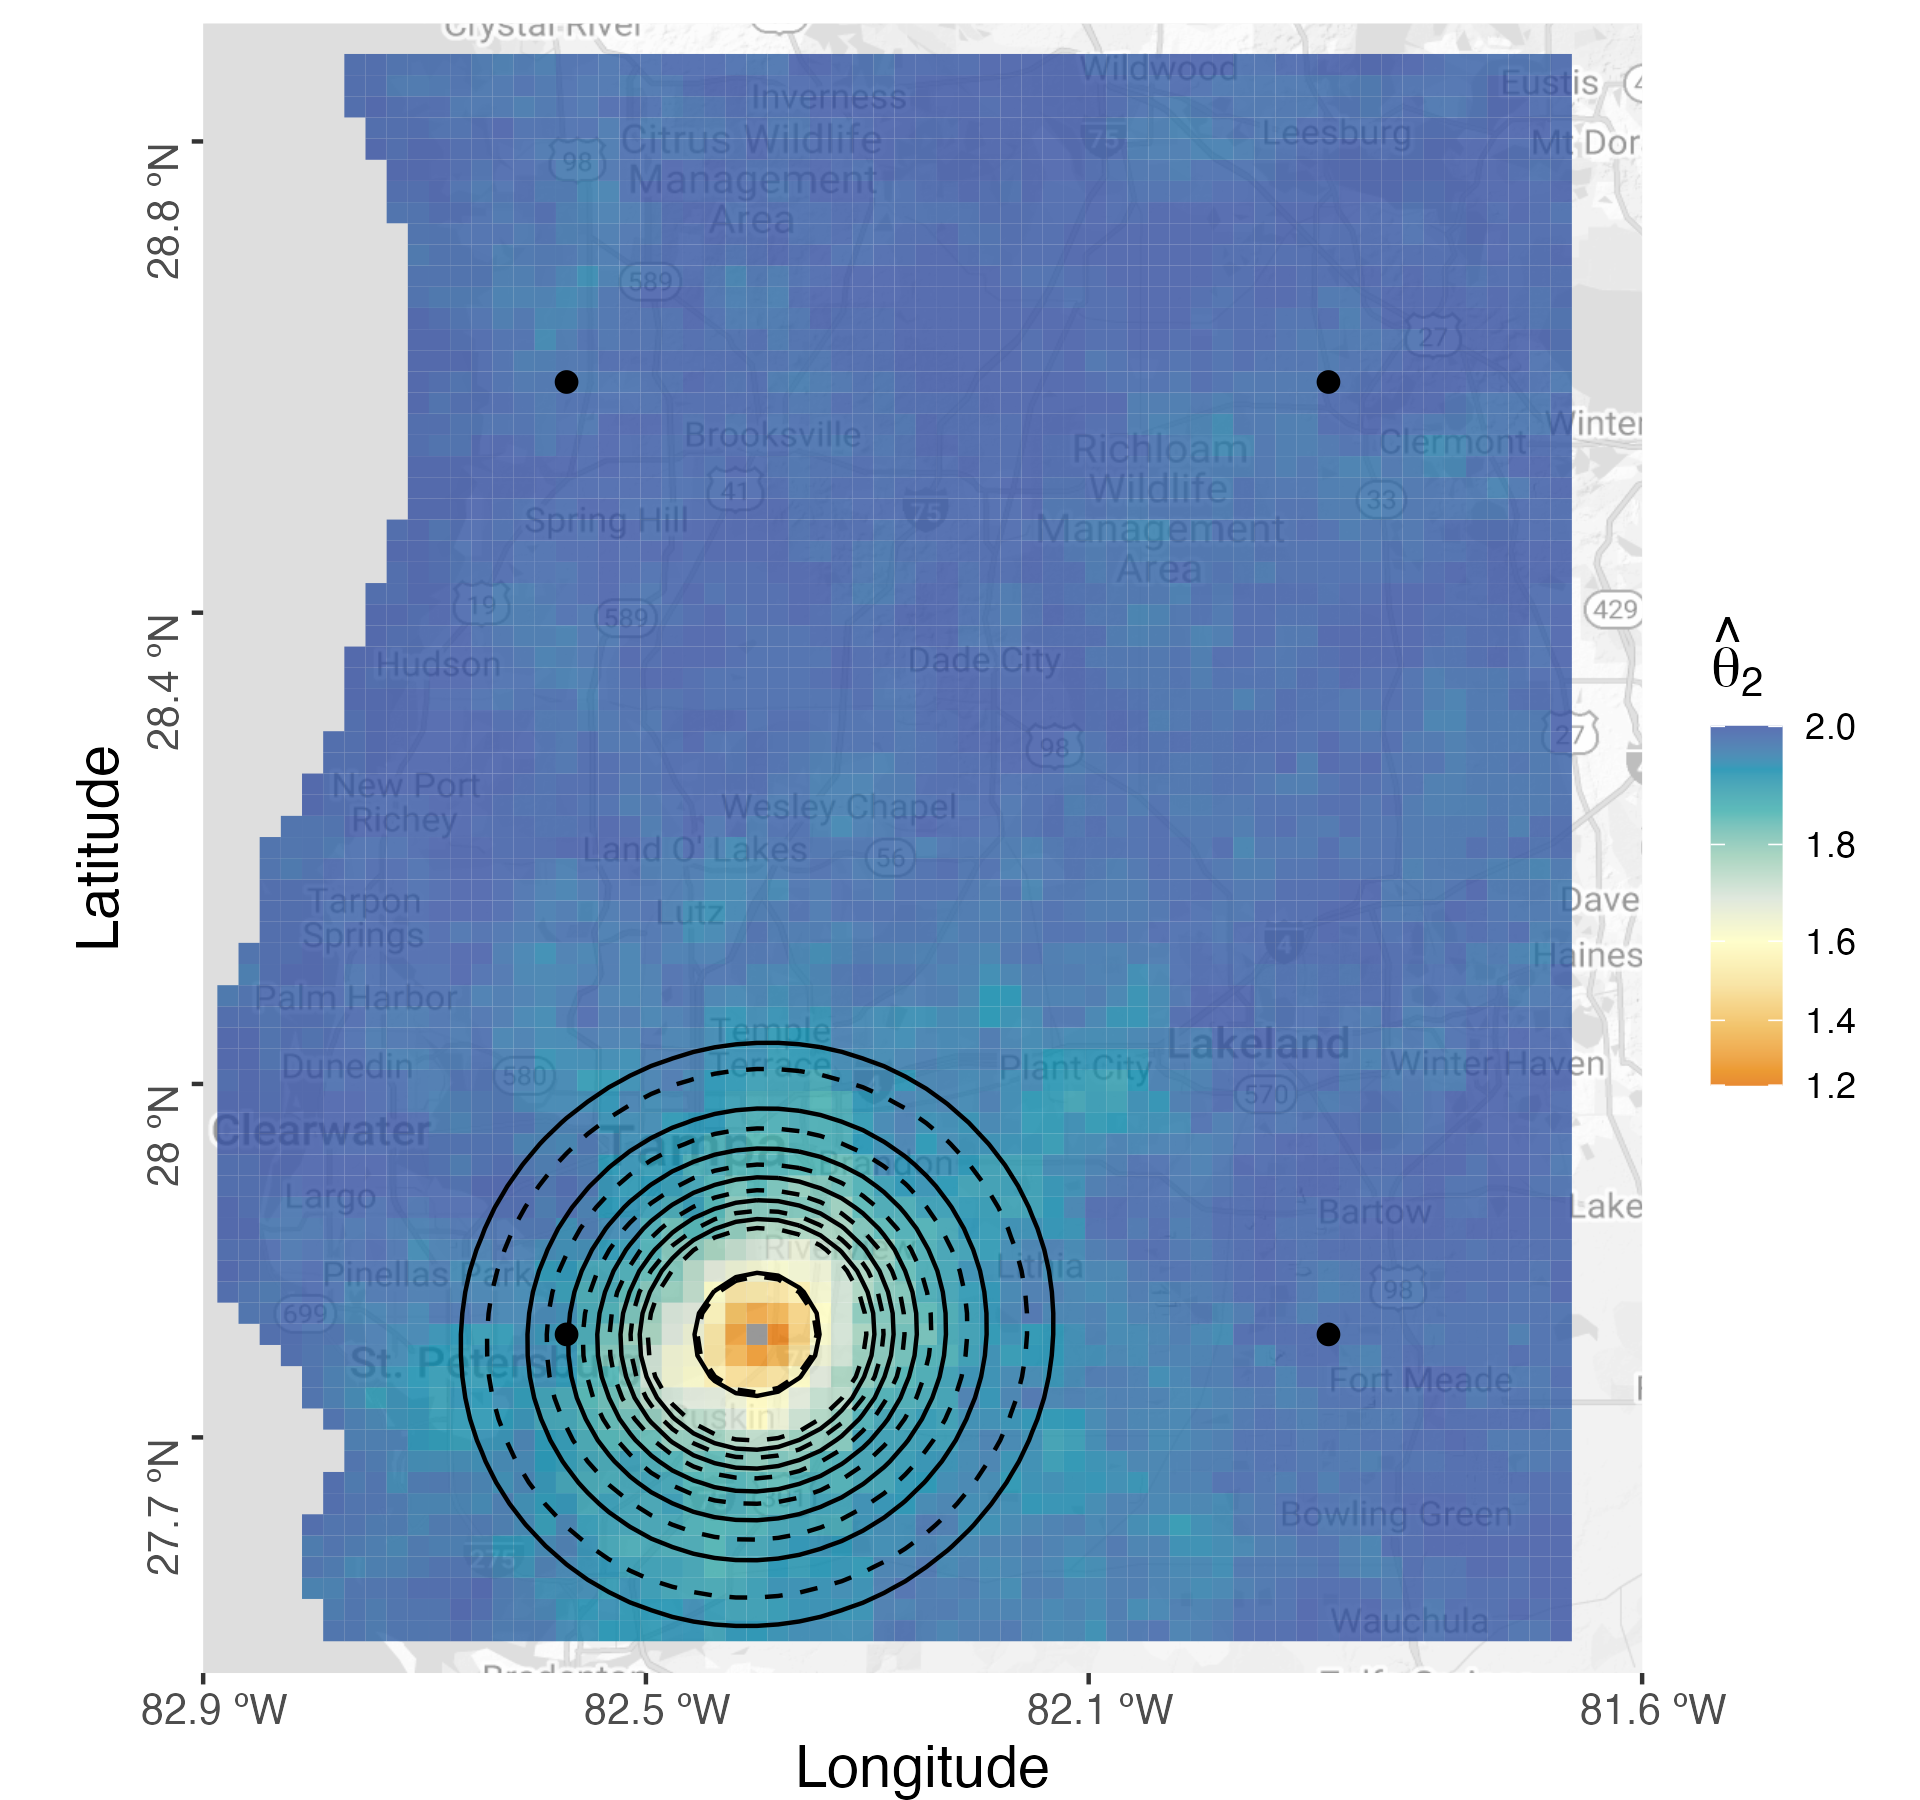
\includegraphics[width=1\textwidth]{florida/florida_extcoef2_2_008.png}
    \end{subfigure}
    \begin{subfigure}{0.45\textwidth}
        \centering
        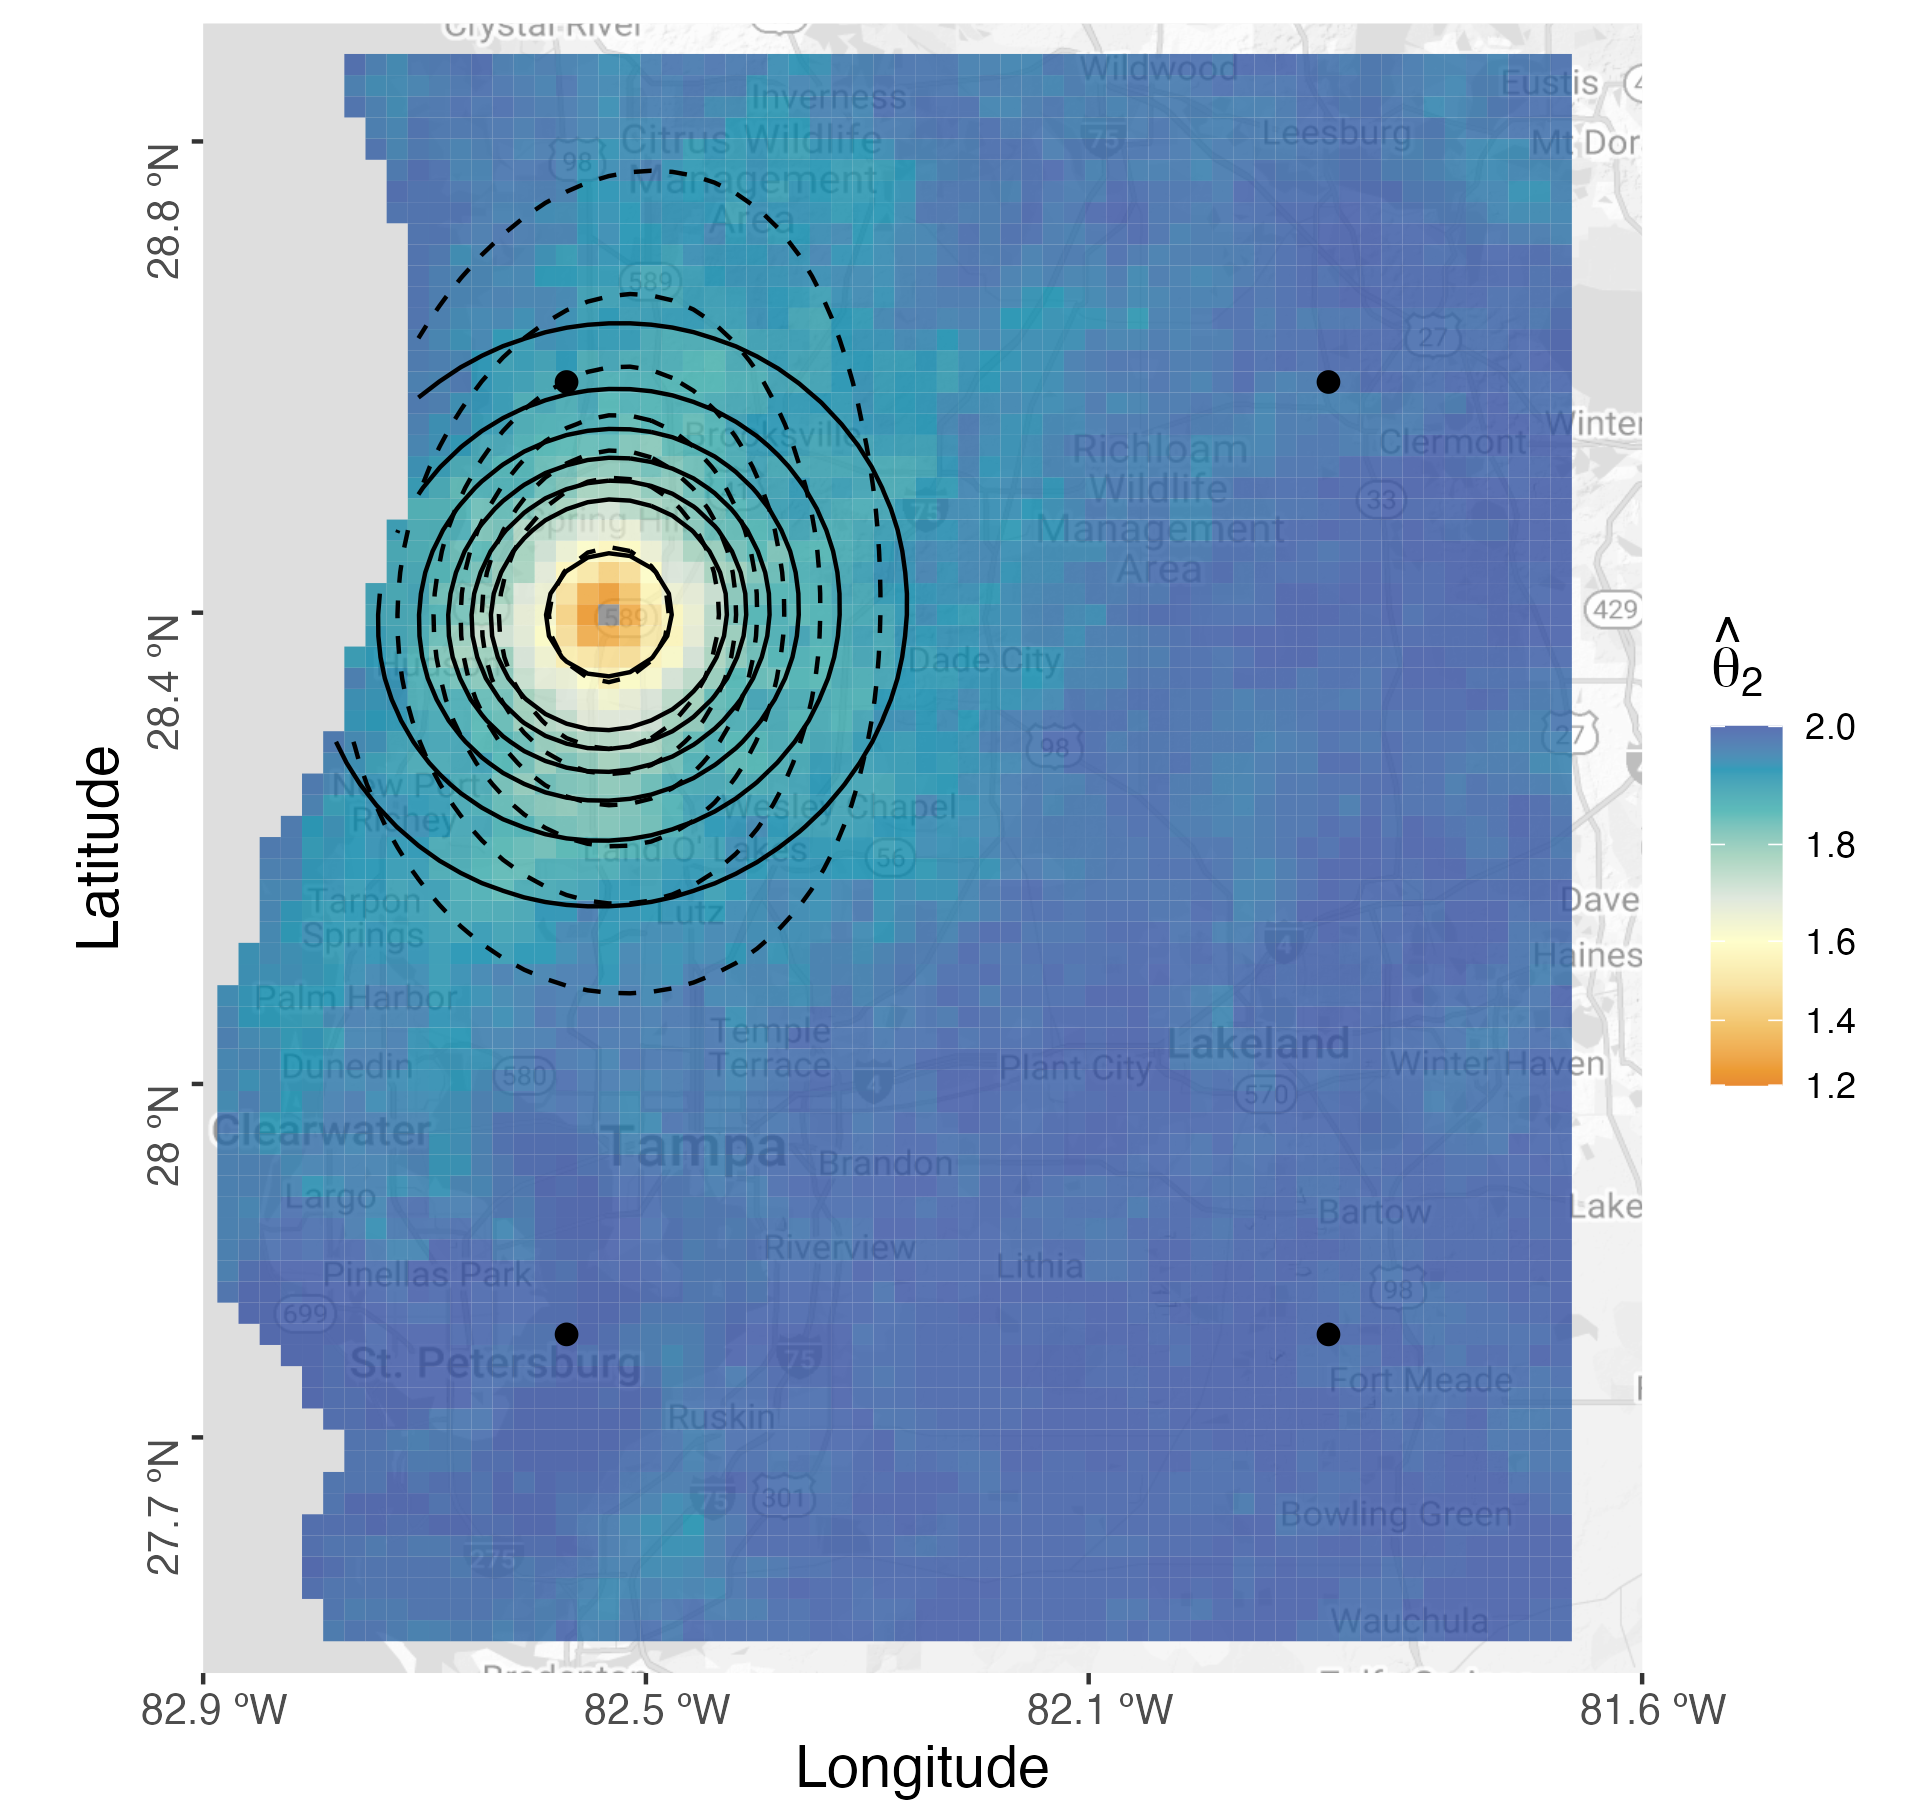
\includegraphics[width=1\textwidth]{florida/florida_extcoef2_2_038.png}
    \end{subfigure}
    \caption{Maps of bivariate empirical extremal coefficients with respect to two different reference point, and contours of the extremal coefficient of the fitted skewed Brown-Resnick (solid line) and Brown-Resnick (dashed line) $r$-Pareto models on the Florida rainfall data. The top and bottom rows respectively consider the $L_1$ and $L_\infty$ norm risk functional. Black dots are the kernel centres used in the skewed Brown-Resnick model.}
    \label{fig:extcoef_application_florida}
\end{figure}


%%%%%%%%%%%%%%%%%%%%%%%%%%%%%%%%%%%%%%%
%%%%%%%%%%%%%%%%%%%%%%%%%%%%%%%%%%%%%%%
\subsection{Analysis of sea surface temperature over the Red Sea}
%%%%%%%%%%%%%%%%%%%%%%%%%%%%%%%%%%%%%%%
%%%%%%%%%%%%%%%%%%%%%%%%%%%%%%%%%%%%%%%

The spatial dependence structure of the sea surface temperature (in $^\circ \textrm{C}$) over the Red Sea is now analysed. Such analysis is critical for risk assessment purposes as it can be leveraged to estimate extreme sea surface temperature hotspots \citep{Hazra.Huser:2021}. Furthermore, some exploratory analysis of the data conducted in \citep{Hazra.Huser:2021} demonstrates the necessity for a model that can capture asymptotic dependence
as well as the presence of non-stationarity in the dependence structure. This positions the proposed skewed Brown-Resnick model as a good candidate to tackle this analysis. 

The data comprises of $31$ annual maxima observations recorded between $1985$ and $2015$ at $D=1,043$ gridded locations.
%
Following the steps detailed in \cite{Huser.Zhong:2023}, the data is pre-processed and the annual maxima are marginally standardized to unit Fr\'{e}chet scale. 
%
The Brown-Resnick and its skewed extension are fitted using the spectral likelihood with threshold $r_0=10\times D$, where $10$ corresponds roughly to the $90\%$ quantile of the unit Fr\'echet distribution, leaving $9$ observations for model fitting.
%
The spline representation of $\bm\eta$ introduced in Section~\ref{ssec:flex_dep} is also chosen here with $5$ kernel centres selected in the middle of the Red Sea, along the North-South axis (see black dots in Figure~\ref{fig:extcoef_application_redsea}). Similarly to the previous analysis, no background noise is added since only $\bm\xi$ needs to be estimated (instead of $\bm\eta$) and the identifiability of $b_i,i=1,\dots,5$ is not a concern. 
%

\cite{Huser.Zhong:2023} define an inference methodology for max-stable processes based on Vecchia approximations which is shown to outperform the composite likelihood approach when applied to the Brown-Resnick model with fixed smoothness parameter $\vartheta$.
%  to avoid difficulties in the joint estimation of the range and smoothness parameters
% In particular, for the dataset under consideration, fixing $\vartheta=1$ proves to be a better choice than $0.5$ or $1.5$.
% , and so did the pairwise over triplewise composite likelihood. 
Motivated by the physical properties of the Red Sea and supported by the model fits, anisotropy is introduced in the (semi)-variogram in a similar way to the previous real data example. 
%
Overall, \cite{Huser.Zhong:2023} concludes that the best results are obtained when fixing $\vartheta=1$ and using a Vecchia approximation with $4$ conditioning sites. This procedure is re-ran with the anisotropic semi-variogram described in \eqref{eq:aniso_mat} and letting parameter $\vartheta$ free. Estimates are obtained in $1.41$ hours and reported in Table~\ref{tab:parameter_estimates_RedSea} (model $\textrm{BR}^v$) and in agreement with those observed by \citet{Huser.Zhong:2023}. 
% with parameter estimates reported to be $\hat{\lambda}=113.9, \hat{\theta} = 0.40$ and $\hat{a}=0.73$ where $a$ is equivalent to $m^2$ in \eqref{eq:aniso_mat} \textcolor{red}{(Peng to confirm)}, and obtained in $5,335$ seconds. 
%
For the composite likelihood, the best reported results consider pairs rather than triples and binary weights with a cut-off distance restricting to first-order neighbours, yielding $2,046$ pairs. This estimation procedure takes $0.93$ hours  which is faster than the Vecchia approximation approach but \cite{Huser.Zhong:2023} note that for the same likelihood complexity, the Vecchia approximation is much faster and already producing better results. 

Focusing on the estimation of the Brown-Resnick parameters, Table~\ref{tab:parameter_estimates_RedSea} indicates statistical efficiency of the spectral likelihood (i.e., model $\textrm{BR}$) is comparable with the composite likelihood and Vecchia approximation approaches but in terms of computational efficiency it is respectively $447\%$ and $729\%$ faster.

% The spectral likelihood approach does not require fixing $\vartheta$ and the Brown-Resnick estimates are \textcolor{red}{$\left( \hat{\lambda}, \hat{\vartheta}\right) = \left(69.04, 1.19\right)$} with jackknife standard deviations \textcolor{red}{$(4.85,0.04)$}, and were obtained in \textcolor{red}{$3.27$} minutes on a single core. 
% 
% Comparatively, the method of \cite{Huser.Zhong:2023} which relies on the pairwise composite likelihood with less than $2,000$ pairs and fixed smoothness parameter $\vartheta$, takes $31$ seconds using 32 cores while fixing the smoothness parameter .
%
\begin{table}[!ht]
    \centering
    \scalebox{0.9}{
        \begin{tabular}{lccccccccccc}
            \hline
           Model & $\hat\lambda$ & $\hat\vartheta$ & $\hat\zeta$ & $\hat m$ & $\hat b_1$ & $\hat b_2$ & $\hat b_3$ & $\hat b_4$ & $\hat b_5$ & \textrm{Time (hrs)}\\ 
            \hline                
            $\textrm{BR}^c$ & 58.61 & 1.35 & -0.54 & 0.76 & - & - & - & - & - & 0.93\\ 
              & (14.79) & (0.18) & (0.05) & (0.04) & - & - & - & - & - \\
            $\textrm{BR}^v$ & 108.91 & 1.16 & 0.79 & 1.21 & - & - & - & - & - & 1.41\\ 
              & (12.20) & (0.09) & (0.10) & (0.06) & - & - & - & - & - \\
            $\textrm{BR}$ & 64.78 & 1.16 & 0.79 & 1.14 & - & - & - & - & - & 0.17\\ 
              & (7.06) & (0.10) & (0.16) & (0.05) & - & - & - & - & - \\  
            sBR & 51.36 & 1.33 & 0.79 & 1.12 & -13.49 & -8.31 & 2.05 & 12.85 & 15.07 & 0.65  \\ 
              & (4.75) & (0.09) & (0.28) & (0.07) & (15.48) & (6.76) & (9.32) & (7.58) & (11.47) & \\ 
            \hline
        \end{tabular}
    }
    \caption{Parameter estimates (jackknife estimates of the standard errors) for the Brown-Resnick (BR) and skewed Brown-Resnick (sBR) max-stable models on the Red Sea, sea surface temperature data. Model name with superscript $v$ or $c$ indicate inference was performed using Vecchia and composite likelihood approximations. No superscript indicate the use of the spectral likelihood.}
    \label{tab:parameter_estimates_RedSea}
\end{table}
%
Fitting the skewed Brown-Resnick model with the spectral likelihood yields a smaller estimate of $\lambda$ and  a larger estimate of $\vartheta$ than for the Brown-Resnick. This is somewhat expected as the fitted skewed Brown-Resnick model better accounts for the dependence strength and structure compared with the Brown-Resnick model. Similarly to the rainfall analysis, the large standard error estimates for the $b_1, \ldots, b_5$ parameters cannot be used to conclude that these parameters aren't useful. On top of the identifiability issues that might be present (but not detrimental to the insights), we recall that only 9 observations of the preocess are used for fitting a 9 parameter model. Looking at the AIC does favour the skewed Brown-Resnick model over the regular Brown-Resnick model ($1843.46$ versus $1871.82$). 
In addition, we note that fitting the skewed Brown-Resnick with the proposed methodology is already faster than fitting the Brown-Resnick using existing approaches.

% \textcolor{red}{[NEED TO RE-RUN MODELS WITH ANISOTROPIC SEMI-VARIROGRAM]}
% The above estimates indicate that the parameters are identifiable, due to the large number of locations and kernel spline used.
% % 
% For the Brown-Resnick model, the parameter estimation takes $196$ seconds on a single core, yielding $\left( \hat{\lambda}, \hat{\vartheta}\right) = \left(69.04, 1.19\right)$ with jackknife standard deviations $(4.85,0.04)$. In comparison, the method of \cite{Huser.Zhong:2023}, relying on the pairwise composite likelihood with less than 2000 pairs, takes $31$ seconds using 32 cores while fixing the smoothness parameter $\vartheta$. In that context, with fixed $\vartheta$ the spectral likelihood takes $57$ seconds using a single core and produces similar results. The skewed Brown-Resnick estimates are $\left( \hat{\lambda}, \hat{\vartheta}, \hat{b_1}, \hat{b_2},\hat{b_3},\hat{b_4},\hat{b_5}\right) = \left(53.12,1.37,-86.99,29.74,-69.96,4.79, 120.59\right)$, which were obtained in 39.5 minutes using 12 cores.
% %with the three-stage optimisation method. 
% The estimated $\hat\lambda$ is smaller but the estimated $\hat\vartheta$ is larger than the corresponding estimates for the Brown-Resnick model, which is to be expected as the estimated skewed Brown-Resnick model more properly accounts for the dependence strength and structure compared with the Brown-Resnick model. The corresponding estimated standard deviations based on the jackknife are $(2.83,0.05,14.08,1.82,1.66,3.37,1.92)$, suggesting that only one of the estimated slant parameters is insignificant.
% % Finally, since the two models are nested, the Akaike Information Criterion can be used for model selection, confirming a better fit when including skewness in the distribution of the underlying process (AIC=-16458.04 versus -16430.1 for the Brown-Resnick).  

To assess the goodness of fit and visualise the differences in dependence structure from the fitted models, Figure~\ref{fig:extcoef_application_redsea} presents maps of the bivariate extremal coefficient for two reference locations. Both maps display some degree of non-stationarity in the dependence structure, in agreement with \citet{Hazra.Huser:2021}, with the contours of the extremal coefficient obtained from the skewed Brown-Resnick being able to capture this phenomena. Together the panels of Figure~\ref{fig:extcoef_application_redsea} give evidence that the extremal coefficient from the proposed model is able to simultaneously characterise the differing behaviour observed in the north and south of the Red Sea, while previous studies had to restrict the modelling to a region at a time \citep[e.g.,][]{Simpson.Wadsworth:2020}


\begin{figure}[!ht]
    \centering
    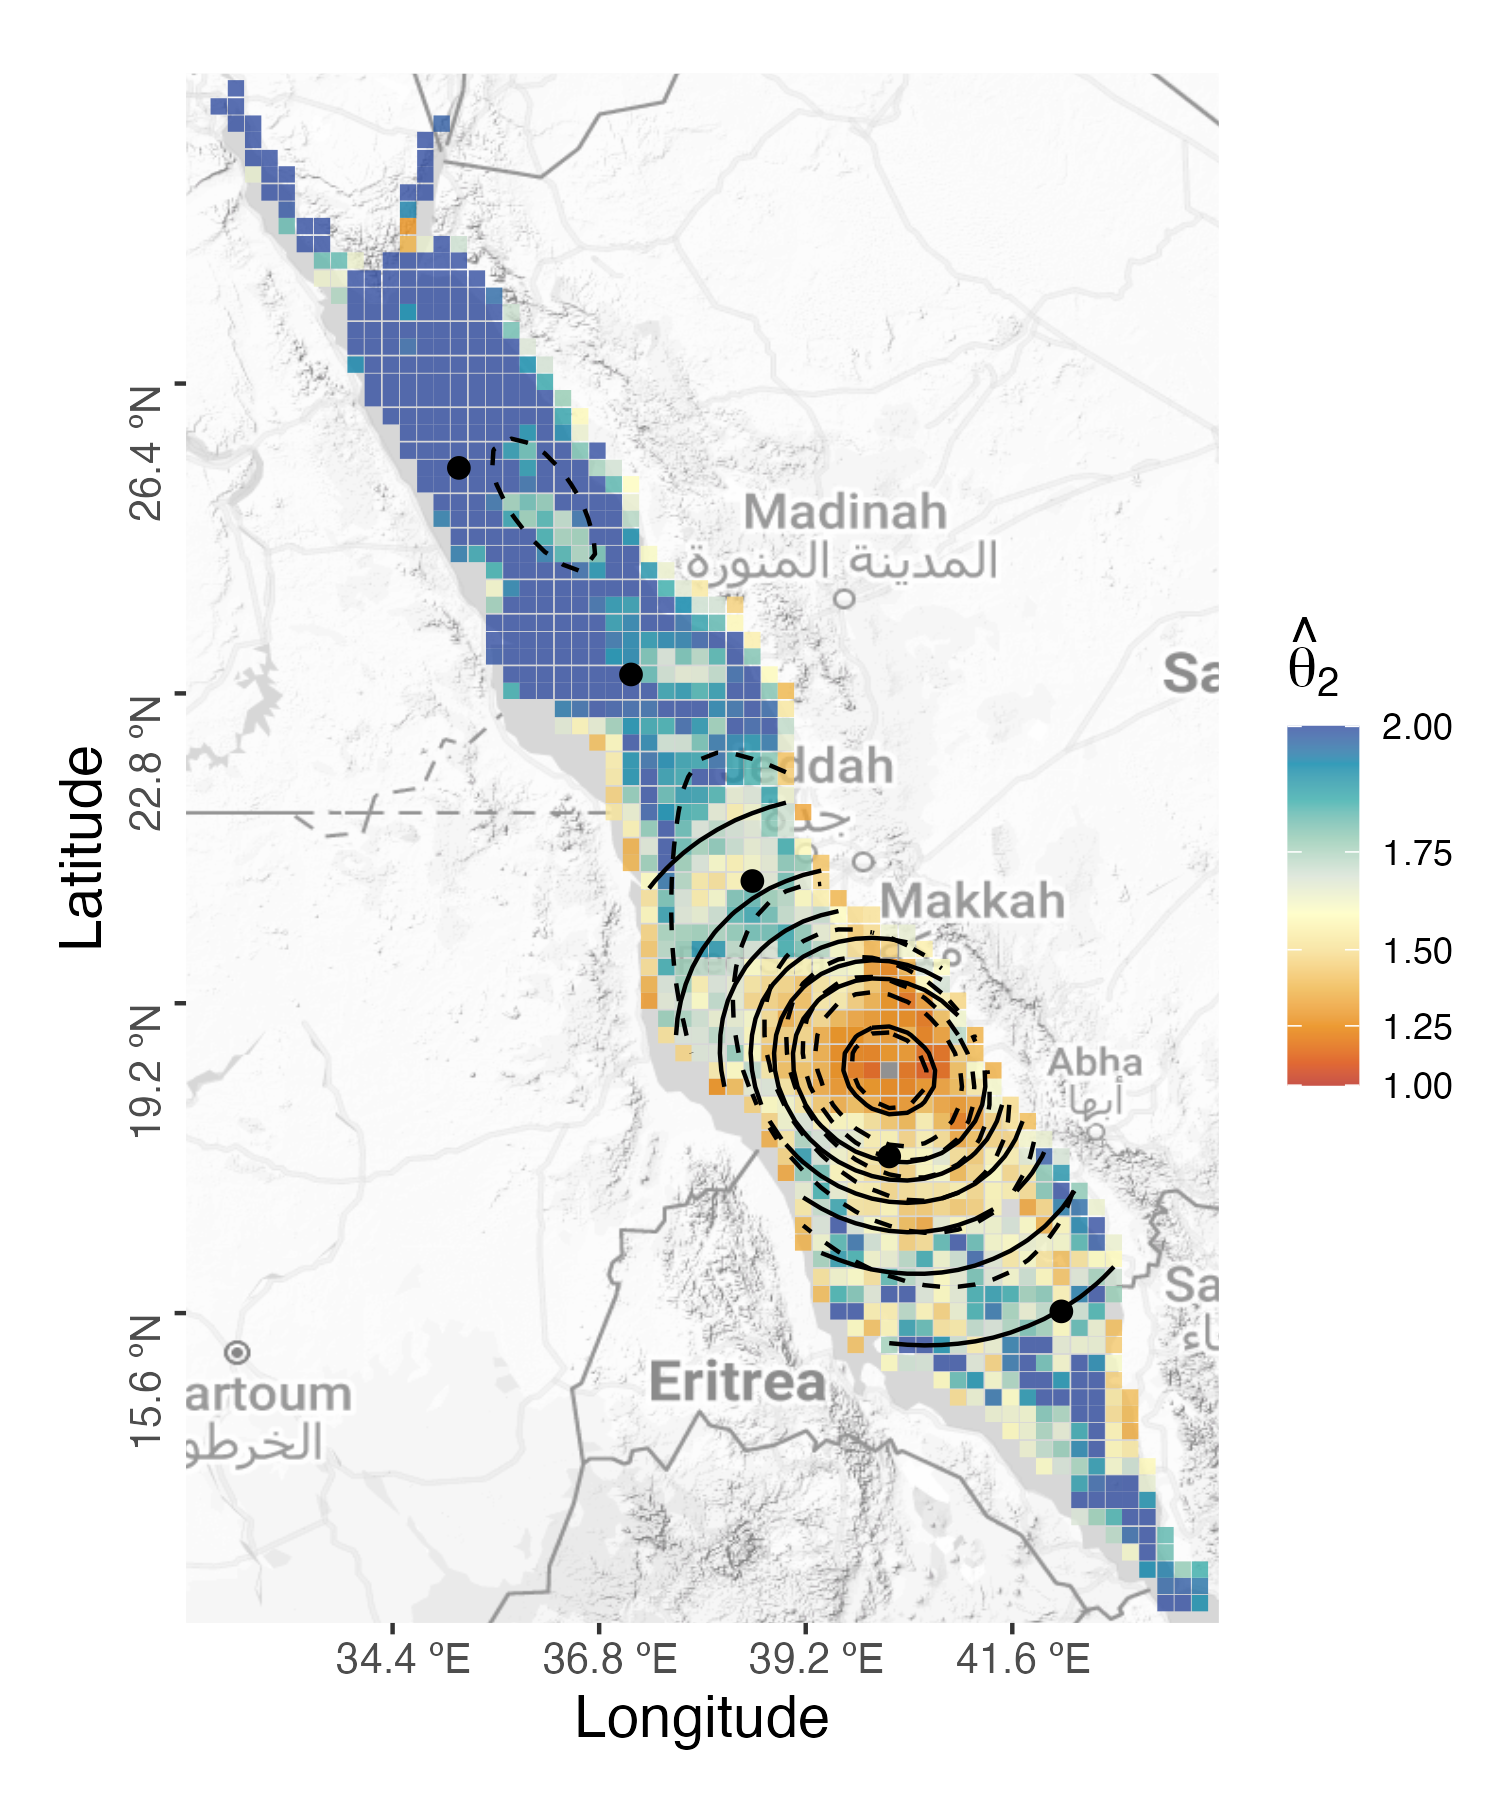
\includegraphics[width=0.49\textwidth]{RedSea2/RedSea_extcoef2_1_035.png}
    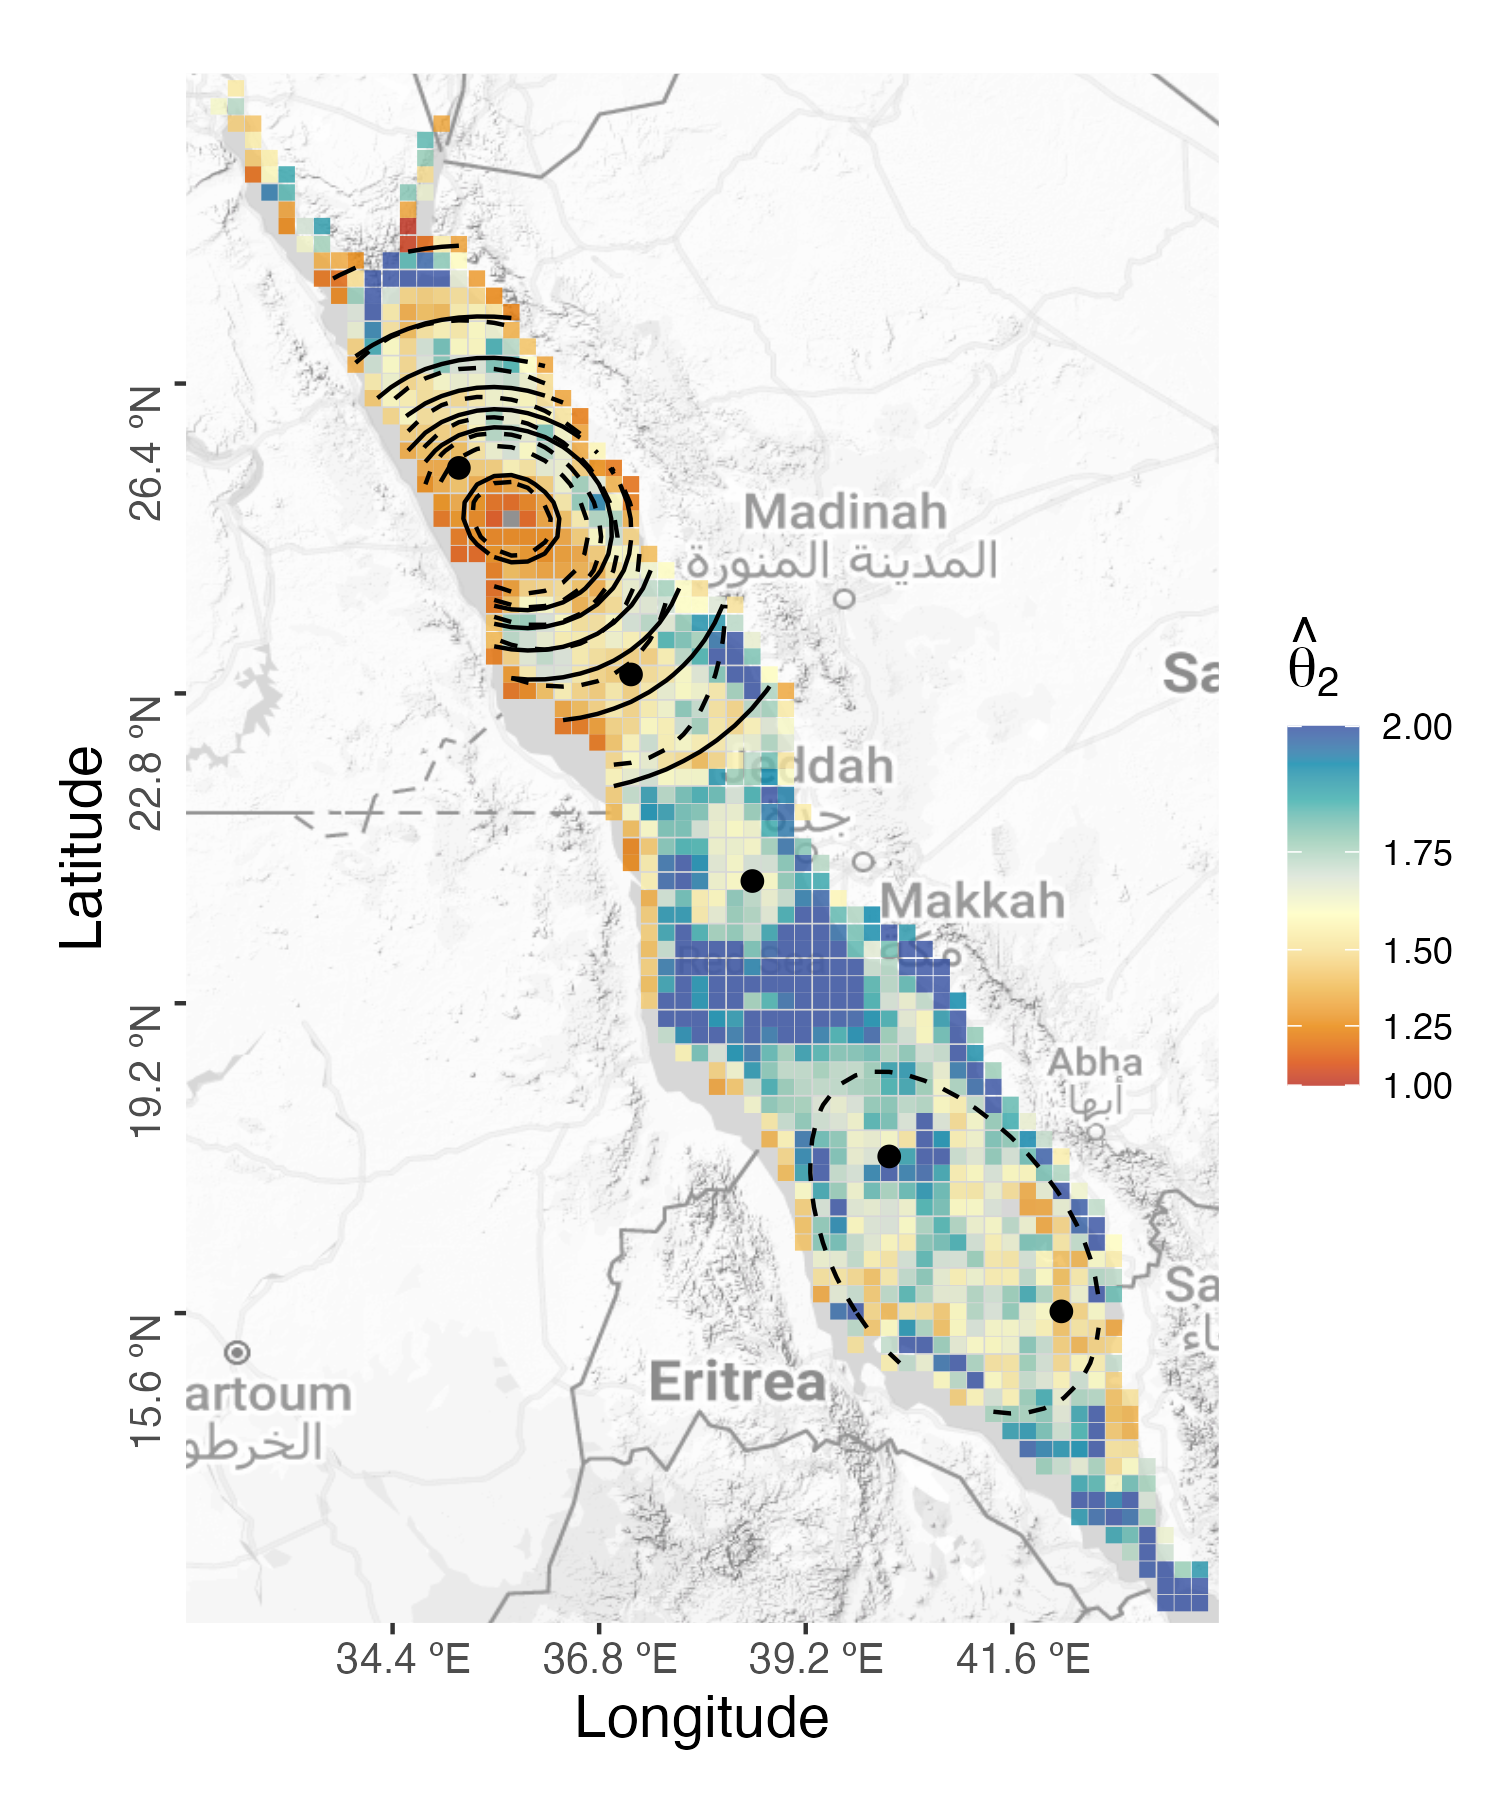
\includegraphics[width=0.49\textwidth]{RedSea2/RedSea_extcoef2_1_082.png}
    \caption{Maps of bivariate empirical extremal coefficient with respect to two reference locations (left and right panels) with contours curves of the estimated extremal coefficients from the Brown-Resnick (solid) and skewed Brown-Resnick (dashed) models. Black dots indicate the kernel centres used in the skewed Brown-Resnick model.}
    \label{fig:extcoef_application_redsea}
\end{figure}

%%%%%%%%%%%%%%%%%%%%%%%%%%%%%%%%%%%%%%%
%%%%%%%%%%%%%%%%%%%%%%%%%%%%%%%%%%%%%%%
%%%%%%%%%%%%%%%%%%%%%%%%%%%%%%%%%%%%%%%
\section{Discussion}
%%%%%%%%%%%%%%%%%%%%%%%%%%%%%%%%%%%%%%%
%%%%%%%%%%%%%%%%%%%%%%%%%%%%%%%%%%%%%%%
%%%%%%%%%%%%%%%%%%%%%%%%%%%%%%%%%%%%%%%

In this article, we establish the condition ensuring the spectral density of a max-stable process only places mass on $\Omega^\circ$, the interior of the $D$-dimensional simplex. This condition directly implies that there is no discontinuities in the associated exponent measure, greatly simplifying the evaluation of the finite dimensional density of the corresponding (generalized) $r$-Pareto process. 

We demonstrate that for models possessing the above property, likelihood-based inference can be done via the spectral likelihood \eqref{eq:angular_likelihood_1}, providing viable solutions to the intractability issues inherent to the likelihood function of max-stable processes and creating opportunities for new $r$-Pareto models. Indeed, out of the two main current models, namely the Brown-Resnick and extremal-$t$, only the former fulfills the condition and is therefore, almost exclusively, the only $r$-Pareto model used in the literature. 

We derive two new models for spatial extremes: the \emph{skewed Brown-Resnick} which offers greater flexibility by allowing for non-stationarity and local anisotropy; and the \emph{truncated extremal-$t$} which mimics the extremal-$t$ while ensuring the continuity condition holds. Exact simulation algorithms for the new max-stable models are provided leveraging existing methodology while a more efficient simulation algorithm for $r$-Pareto processes is established. 

For a sufficiently high threshold, the inference approach is shown to have moderately biased estimates for max-stable models and unbiased estimates in the $r$-Pareto case. In addition, unlike competing estimation procedures (composite likelihood and score matching), the spectral likelihood is able to estimate reasonably well the slant parameters of the skewed Brown-Resnick. Through simulation experiments we highlight that, together with its ability to correctly estimate model parameters, the approach also provides major computational gains over composite likelihood and score matching alternatives.

The need for better, more flexible models is illustrated on both threshold exceedances and annual maxima data, providing new insights about the non-stationary dependence structure of respectively extreme precipitation and sea surface temperature levels. The proposed methodology is proven to be computationally more efficient that state of the art methodology such as score matching \citep{deFondeville.Davison:2018} and Vecchia approximation \citep{Huser.Zhong:2023}, allowing to deal with much higher dimensional datasets. Overall, this manuscript offers theoretical and methodological advances resulting in better and faster characterisation of spatial extremes events.


% We have proposed a class of models for spatial extreme modeling whose spectral density does not have mass on the boundary space and avoids computing partial derivatives of the exponent function, the number of which quickly becomes intractable as the dimension of the data increases. 
% %In particular, the methodology can easily be applied to very high dimensional data under the condition that the spectral density only puts mass on the interior of the unit simplex $\Omega$ and, as such, 
% We have established general conditions for a model to possess such property. The well-known Brown-Resnick process falls within this family of models and we derive two new extreme models: the \emph{skewed Brown-Resnick}, an extension of the Brown-Resnick that can model non-stationarity and local anisotropy, and the \emph{truncated extremal-t}, the equivalent of the extremal-t but without mass on the subspaces of the simplex.  

% Our simulation experiments have verified that, given an appropriately chosen threshold for the radial component, the spectral likelihood can perform as well as the pairwise composite likelihood and in some instances better, especially for our new skewed Brown-Resnick model, since pairwise likelihood cannot pick up the local anisotropic dependence structure. As for r-Pareto processes, the score matching method is highly numerical unstable to produce reasonable estimates compared to the spectral likelihood method. The statistical efficiency of the methodology is paired with its computational efficiency which allows it to fit flexible models to dimensions in thousands, as illustrated on a real dataset, within a reasonable timeframe. The advantages of the proposed methodology over the recent work of \citet{Huser.Zhong:2023} are also highlighted. Overall, this approach will help expand the usability of the asymptotic extreme models including max-stable and r-Pareto models in practice.  

The new models introduced in this manuscript are also a step closer towards building spatial extreme models suited for real-world problems and expanding the class of extremal graphical models with flexible dependence structures as the only graphical extreme models are currently built upon the Brown-Resnick model or H\"usler-Reiss model \citep{Engelke.Hitz:2020,Hentschel.Engelke.Segers:2024,Wan.Zhou:2023}. 

%%%%%%%%%%%%%%%%%%%%%%%%%%%%%%%%%%%%%%%
%%%%%%%%%%%%%%%%%%%%%%%%%%%%%%%%%%%%%%%
%%%%%%%%%%%%%%%%%%%%%%%%%%%%%%%%%%%%%%%
\section*{Supplemental Material}
%%%%%%%%%%%%%%%%%%%%%%%%%%%%%%%%%%%%%%%
%%%%%%%%%%%%%%%%%%%%%%%%%%%%%%%%%%%%%%%
%%%%%%%%%%%%%%%%%%%%%%%%%%%%%%%%%%%%%%%

The Supplemental Material contains the proofs of the theorems and propositions, and the exact simulation algorithms for the skewed Brown-Resnick and truncated extremal-t models. The code for the simulation study and the application is available at \url{https://github.com/PangChung/InteriorExtremes}. 

%%%%%%%%%%%%%%%%%%%%%%%%%%%%%%%%%%%%%%%
%%%%%%%%%%%%%%%%%%%%%%%%%%%%%%%%%%%%%%%
%%%%%%%%%%%%%%%%%%%%%%%%%%%%%%%%%%%%%%%
\section*{Acknowledgements}
%%%%%%%%%%%%%%%%%%%%%%%%%%%%%%%%%%%%%%%
%%%%%%%%%%%%%%%%%%%%%%%%%%%%%%%%%%%%%%%
%%%%%%%%%%%%%%%%%%%%%%%%%%%%%%%%%%%%%%%

This work was supported by the Australian Research Council (ARC) through the Discovery Project Scheme (DP220103269). 

\baselineskip=18pt
\bibliographystyle{CUP}
\bibliography{Total.bib}

\end{document}
